\documentclass[10pt,b5paper,twoside]{article} 
\usepackage[latin1]{inputenc}
\usepackage[english]{babel}
\usepackage{amsmath}
\usepackage{amsfonts}
\usepackage{amssymb}
\usepackage{makeidx}
\usepackage{graphicx}
\usepackage{hyperref}
\usepackage[left=2cm,right=2cm,top=2cm,bottom=2cm]{geometry}
\usepackage{float}
\usepackage{multirow}
\usepackage{verbatim} %for å kommentere ut ting
\usepackage[nottoc,numbib]{tocbibind}
\usepackage{chngpage} % allows for temporary adjustment of side margins
\usepackage[parfill]{parskip} %for avsnitt
\usepackage{listings}
    \lstset{
            language=Matlab,                                % choose the language of the code
    %       basicstyle=10pt,                                % the size of the fonts that are used for the code
            numbers=left,                                   % where to put the line-numbers
            numberstyle=\footnotesize,                      % the size of the fonts that are used for the line-numbers
            stepnumber=1,                                           % the step between two line-numbers. If it's 1 each line will be numbered
            numbersep=5pt,                                  % how far the line-numbers are from the code
    %       backgroundcolor=\color{white},          % choose the background color. You must add \usepackage{color}
            showspaces=false,                               % show spaces adding particular underscores
            showstringspaces=false,                         % underline spaces within strings
            showtabs=false,                                         % show tabs within strings adding particular underscores
    %       frame=single,                                           % adds a frame around the code
    %       tabsize=2,                                              % sets default tabsize to 2 spaces
    %       captionpos=b,                                           % sets the caption-position to bottom
            breaklines=true,                                        % sets automatic line breaking
            breakatwhitespace=false,                        % sets if automatic breaks should only happen at whitespace
            escapeinside={\%*}{*)}                          % if you want to add a comment within your code
    }

\raggedbottom

\usepackage{makeidx}
\makeindex
%symbolliste slutt

\author{Anders Dall'Osso Teigset}
\title{MEDIUM VOLTAGE LOAD BREAK SWITCH WITH AIR AS INTERRUPTING MEDIUM}
\date{December, 2013}


\begin{document}
    \begin{titlepage}
    \begin{center}
    \ \\
    \ \\
    \ \\
    \ \\
    \ \\
    \ \\
    Anders Dall'Osso Teigset \\
    \ \\
    \ \\
    \ \\
    \ \\{\large \bfseries
    MEDIUM VOLTAGE LOAD BREAK SWITCH WITH AIR AS INTERRUPTING MEDIUM\\
    }
    \ \\
    \ \\
    \ \\
    \ \\
    \ \\
    {\large
    Specialisation project\\
    }
    \ \\
    {December, 2013 \\}
    \ \\
    \ \\
    \ \\
    \ \\
    \ \\
    \ \\
    \ \\
    \ \\
    \ \\
    \ \\
    \ \\
    \ \\
    \ \\
    \ \\
    \ \\
    \ \\
    \ \\
    \ \\
    \ \\
    \ \\
    \ \\
    \ \\
    \ \\
    \ \\
   	{\large
   Norwegian University of Science and Technology\\
   Department of Electric Power Engineering\\
    }
   	\ \\
    \ \\
    \end{center}
    \end{titlepage}

%\maketitle
%SummaryNyttige pdf-filer/SF6conduct.pdf
\thispagestyle{empty}
\cleardoublepage
\section*{Acknowledgements}
\setcounter{page}{1}
\pagenumbering{roman}

\cleardoublepage
\section*{Summary}

\cleardoublepage
\setcounter{page}{1}
\pagenumbering{arabic}
\tableofcontents
\cleardoublepage

\section{Introduction}

\cleardoublepage

\section{Theory}
\subsection{Typical switchgear design and interruption sequence} \label{sec:genDes}
Most of the information in section \ref{sec:genDes} is collected from \textit{"Current Interruption in Power Grids"} by Magne Runde \cite{bib:HVEbreak} \newline

\subsubsection{Switchgear design and operation} \label{sec:InterruptCurrent}
Switchgear can be divided into four main categories:
\begin{itemize}
\item Disconnector Switch
\item Load Break Switch
\item Circuit Breaker
\item Earthing Switch
\end{itemize}

This report will focus on the load break switch (LBS) design. An LBS is designed to be able to interrupt currents with a magnitude equal to or less than the rated maximum continuous current in a transmission system. An LBS should fulfil the following demands in order to meet the requirements of the application area:

\begin{itemize}
\item When closed:
	\begin{itemize}
		\item Act as a good conductor.
		\item Be capable of interrupting any load that may arise, without generating too high over-voltages. 
	\end{itemize}
\item When open:
	\begin{itemize}
		\item Act as a good insulator.
		\item Be able to close without welding the contacts together, even under short-circuit conditions.
	\end{itemize}
\end{itemize}

A typical opening sequence for a switch is as follows: First, a control signal enters the switch and activates the driving mechanisms. In most cases, this is a compressed spring or a hydraulic system. The contacts begin to open, and a gap forms between them. At the same time, an electrical arc ignites between the contacts, burning in the gap. The gap is filled with some kind of interrupting medium which is usually a gas. When an altering current crosses zero, this is referred to as the current zero (CZ). For an alternating current with a frequency of 50 Hz, CZ will occur 100 times per second. Direct current interruptions will not be explained in this report.

%bilde som viser driving mechanisms compressed spring contacts?

At the CZ, the arc will extinguish for at least a moment, because the current is zero, and a voltage will build up between the contacts. This voltage is called the recovery voltage, and is defined in equation \eqref{eq:U_rec}, where $u_{supply}$ is the voltage on the supply side and $u_{load}$ is the voltage on the load side of the open switch. Depending on the recovery voltage two possible scenarios can occur: a re-ignition or a successful quenching of the arc. This is dependent on the steepness and the amplitude of the recovery voltage. There are two different kinds of re-ignition: thermal and dielectric. Thermal re-ignition takes place right after CZ, up to a few microseconds, and is mainly dependent on the steepness of the recovery voltage. As the recovery voltage rises and if a thermal re-ignition is avoided, a dielectric re-ignition may occur. This kind of re-ignition is largely dependent on the amplitude of the recovery voltage, and will occur after a millisecond or more. This paper will mainly focus on thermal re-ignition. The likelihood of a re-ignition  will not be de-terminated by the arcing voltage itself, but by how the interrupting medium used reacts on the arcing voltage. Important interruption properties of air is featured in section ???. Other design parameters like contact material, geometry, speed of the contact movement, and cooling mechanisms are also important to the interruption properties.

\begin{equation} \label{eq:U_rec}
u_\mathrm{{recovery}}=u_\mathrm{{supply}}-u_\mathrm{{load}}
\end{equation}  

The plasma state of an interrupting medium occurs when gas and metal vapour are heated to very high temperatures. At a certain point, the molecules in the gas decompose to ions and free electrons. This mixture is called plasma, and it makes up for most of the components in which an electrical arc burns, except for arcs that burns in vacuum. Plasma is an ideal electrical conductor compared to gas, which is an insulator. Vacuum arcs will not be featured in this report.

In most switchgear designs, it is common to have two contact sets: one called the main contact and another called the arcing contact. The main contact is the first contact to open and the last one to close. This is to ensure that an arc does not start to burn between the main contact. The arcing contact is the last contact to open, and the first one to close, and will ensure that the arc burns between the arcing contact and never between the main contact.

Since the main contact opens first and closes last, its main purpose in the switchgear is to act as a good conductor. Copper or aluminium are good materials, and are commonly used to ensure that this aspect of the switch is met. Sometimes, the contact surface is plated with tin, gold, silver, or platinum in order to ensure an even lower contact resistance between the contacts. The main problem with electrical losses in the switch is heat generation, which may speed up metal creep and other ageing-related processes in the switch. Contacts made of aluminium are especially vulnerable to creeping.

The arcing contacts are designed to withstand the harsh conditions that occur when an arc burns between the contacts. The contact material has to meet strict requirements, and has to tolerate high temperatures and arc erosion, and avoid welding and other stresses that may apply when closing or opening an energized contact. Aluminium and copper are not fit for these tasks, since they will melt or erode from the stresses of an arc. It is common to use composites that consist of metals with good electrical conduction and heat-resistant oxides. For high current and voltage switches, it is possible to use a composite of silver or copper together with tungsten or tungsten carbide. These materials are highly heat-resistant, but they also have a high electrical resistance. The higher electrical resistance in the arcing contact compared to the main contact is, however, not a problem, since the current only flows through the arcing contact for a short period of time.

\subsubsection{The puffer principle} \label{sec:puffer}
In order to quench the arc, several mechanisms and interrupting mediums can be applied. In a compact LBS based on SF$_6$, the puffer mechanism is often used. In order to obtain a successful interruption of an arc, the arc and interruption medium must be cooled down, and the charged particles and vaporised metal between the arcing contacts must be blown off. This is the main purpose of the puffer mechanism. The puffer mechanism is based on a piston, and it generates a gas flow in the switchgear in order to extinguish the arc. A typical design of this system consists of a fixed piston integrated inside the movable contact part. A gas reservoir trapped between the arcing contact and the piston is pushed out as the contact move apart from each other. Figure \ref{fig:CircutBreakPuff1} displays a typical puffer design.

When SF$_6$ entered the industry in the 1960s, it was in the form of dual pressure breakers. The SF$_6$-based dual pressure breakers had one high pressure chamber, and one low pressure chamber. A valve from a high pressure chamber opened during opening operations, generating a high speed SF$_6$ blast, guided by a nozzle to hit the arc burning between the contacts in the low-pressure chamber. This design has two major disadvantages when using SF$_6$. The switch requires heating in order to maintain the pressure in the high-pressure chamber for preventing condensation of the SF$_6$ gas. It also uses a compressor for pumping the gas from the low-pressure chamber to the high-pressure chamber. This adds to the complexity of the switchgear, and may result in more maintenance. The double pressure design was replaced with the newer single pressure design. The single pressure design has only one pressure chamber with low pressure, except during interruptions, when the chamber itself becomes a high-pressure chamber.

The single pressure design uses a puffer or the self-blast mechanism to quench the arc, or in some cases a combination of both. The self-blast mechanism is a concept that uses the expansion of the gas for creating a pressure difference and a gas flow to cool the arc. Common for both puffer and self-blast mechanisms is that they do not use a compressor to generate the gas flow, but uses the energy stored in the switching mechanisms or generated from the blast itself to interrupt the arc. These mechanisms work the same way for both circuit breakers and load break switches, but will in a load break switch be smaller and less complex. This is because the current amplitudes are smaller, and therefore a lower pressure is needed to obtain a successful interruption.

\begin{figure} [H]
\centering
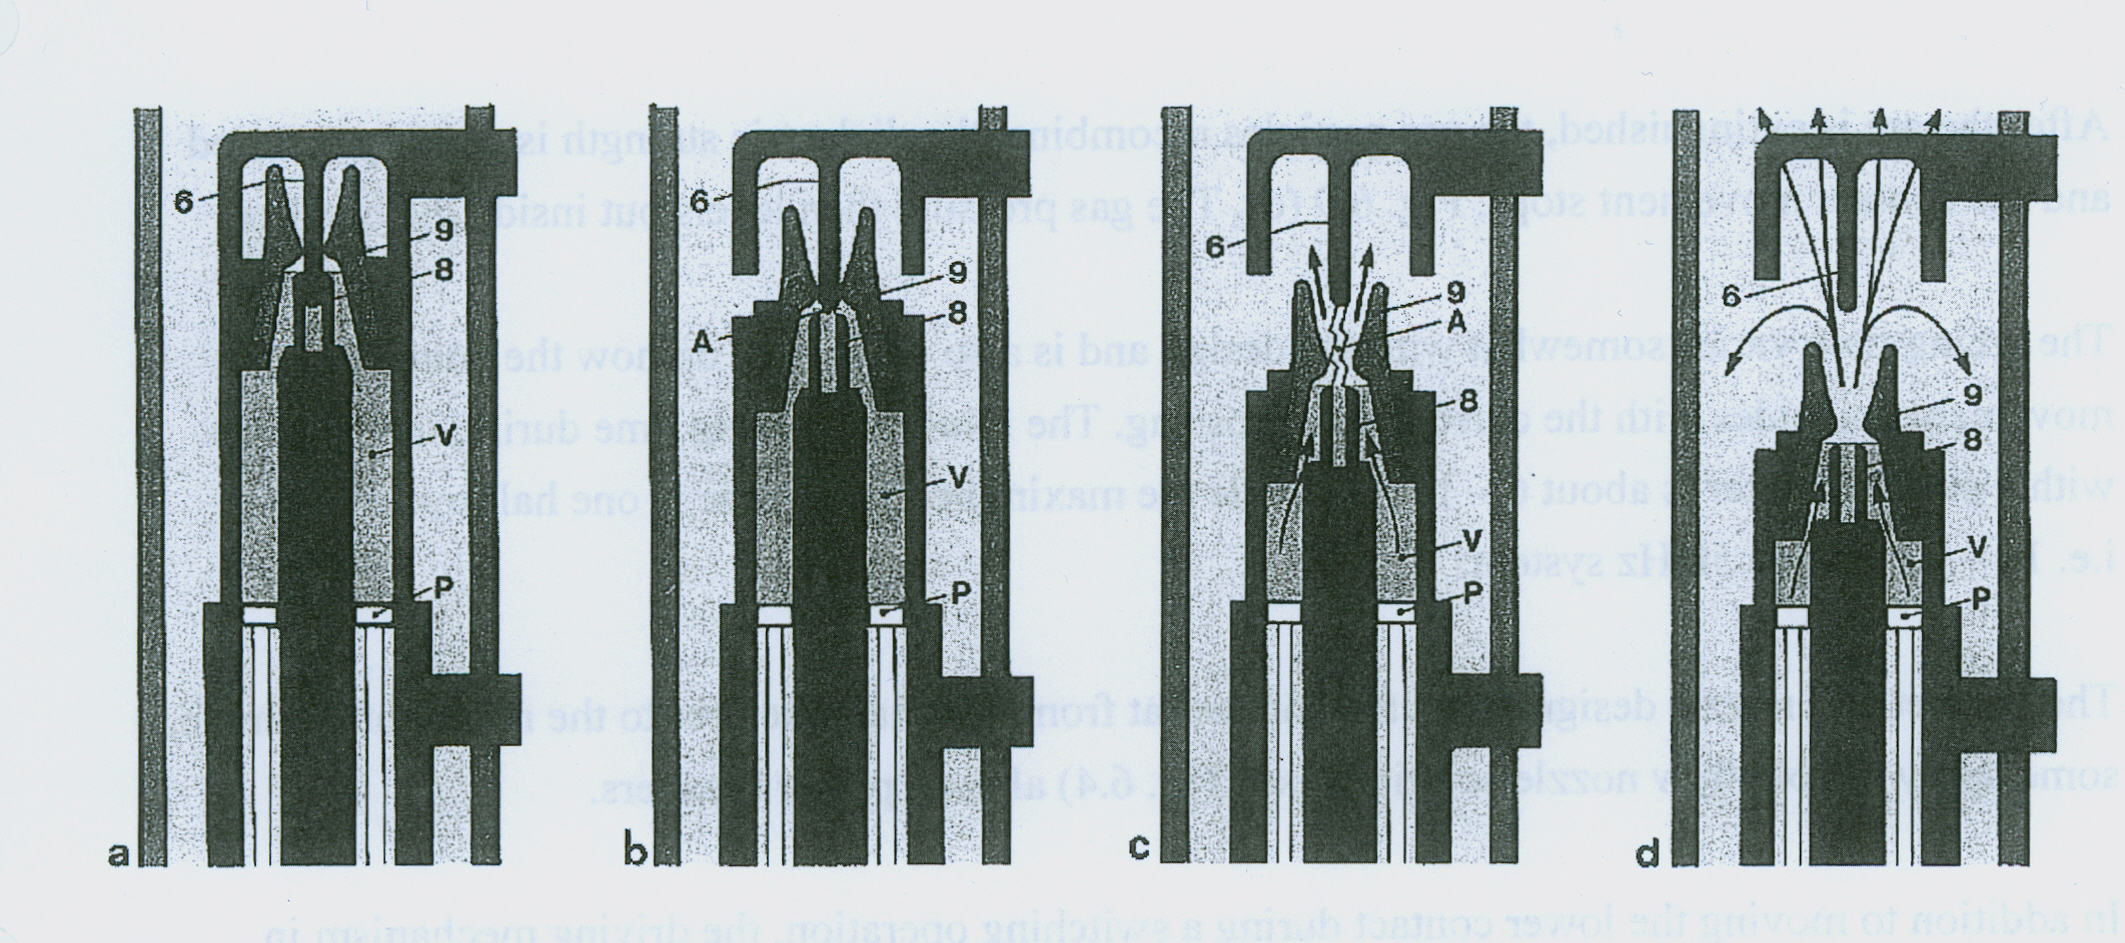
\includegraphics[scale=0.75]{Bilder/Theory/CircutBreakPuff1.png}
\caption{Interruption sequence in a breaker using the puffer mechanism \cite{bib:HVEbreak}.} \label{fig:CircutBreakPuff1}
\end{figure}

Figure \ref{fig:CircutBreakPuff1} displays a typical interruption sequence of a breaker based on the puffer design. When the breaker is closed, as illustrated in figure \ref{fig:CircutBreakPuff1}a, a gas volume \textit{(V)} is trapped between the piston \textit{(P)} and the arcing contact, \textit{(8)} and \textit{(6)}. During the period of time where the movable part of the arcing contact \textit{(8)} is pulled down, the volume decreases because of the placement of the fixed piston, and the pressure increases due to compression of the gas. Figure \ref{fig:CircutBreakPuff1}b illustrates the situation where the main contact is open and the current now only flows through the arcing contact.

The next stage of the interruption sequence is shown in figure \ref{fig:CircutBreakPuff1}c. The arcing contacts have now separated, and an arc \textit{(A)} has ignited between the contacts. The pressurised gas that previously was trapped between the piston and the arcing contact is now released. A nozzle \textit{(9)} that is fixed to the movable arcing contact guides the gas flow so that it will cool the arc down and blow away charge carriers between the contacts. If a sufficient gas flow is obtained, the arc will neither re-ignite after current zero, nor extinguish before current zero.

The gas flow is partially dependent on the cross-section of the arc, which again is dependent on the current amplitude. A large current resulting in a large arc may block the hole in the nozzle, preventing a gas flow. This is called current clogging, and may occur for certain nozzle designs at high current interruptions. In such an event, the pressure in the gas reservoir will increase further due to compression from mechanical moment of the arcing contact and thermal expansion in the gas, because of heating from the arc. When the current amplitude approaches zero, its cross-section will decrease and the clogging effect will end. This will result in a powerful gas blast onto the arc, as indicated in figure \ref{fig:CircutBreakPuff1}d. For smaller current amplitudes, the arc cross-section is smaller, and a clogging effect does not occur to the same extent. This generates a less intense gas flow, preventing the current from being interrupted before its natural zero crossing.

The self-blast, or third generation breaker, was developed with the goal of reducing mechanical power of the operating system, making it cheaper and less complex. Figure \ref{fig:selfBlast} illustrates the working principle of a breaker using self-blast to interrupt an arc. The difference between self-blast and puffer mechanism is that the puffer mechanism increases the pressure by reducing the volume, while the self-blast design has a constant volume and relies on a rise in temperature to increase the gas pressure \cite{bib:CBAC}. The self-blast design uses the heat generated from an arc burning between the arcing contacts to interrupt the current. The gas expands as it is heated by the burning arc. This increase in pressure leads to a gas flow on the arc, which cools it down, leading to the arc being quenched.

\begin{figure} [H]
\centering
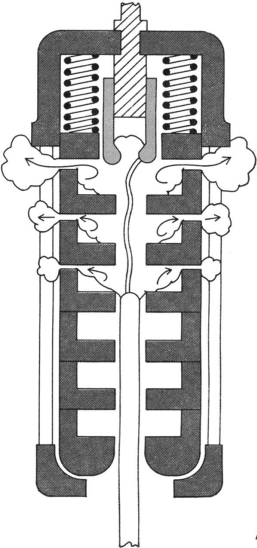
\includegraphics[scale=0.33]{Bilder/Theory/selfBlast.png}
\caption{Expulsion chamber in a breaker using the self-blast mechanism \cite{bib:CBAC}.} \label{fig:selfBlast}
\end{figure}

There are some disadvantages of the self-blast principle when compared to the puffer mechanism. The self-blast has a lower dielectric strength, due to hot gas between the contacts after CZ. This gives a higher chance of re-ignition since hot gas has lower ionisation energy than cold gas. The design is also not well suited to break smaller currents. This is because the arc is less intense and therefore does not heat the gas sufficiently to create a strong enough blast. Therefore, it is common to combine self-blast and puffer mechanism in a hybrid design, so that it can handle both small and large currents. A compact LBS design using air as interrupting medium will probably rely on a puffer design. This is because an LBS faces smaller currents than a circuit breaker.

A good circuit breaker design is considered hard to develop, and the industry needs to optimise the product to meet the demands set by the market, such as size and pressure. This is due to high short-circuit current in the range of 40 kA and large recovery voltages. Because of this, the industry has put a lot of effort into circuit breaker development. Nonetheless, when designing an LBS based on SF$_6$, it is common to take the working principle of a circuit breaker and scale it down to a suitable size for an LBS, and then test it. If it works, the LBS might be sold on the market without further alterations. When using air, this development technique has not been implemented successfully, since higher demands are set to the interrupting capabilities of the switchgear. This is because SF$_6$ is superior to air as an interrupting medium and the behaviour of the arc also alters with the current. However, the same interruption techniques might be used, but with an increased focus on optimisation. In figure \ref{fig:selfBlastandPuffer}, the interrupter of a load break switch is shown. This is a down-scaled version of a circuit breaker, which has successfully been used to interrupt load current with SF$_6$ gas as interruption medium. 

\begin{figure} [H]
\centering
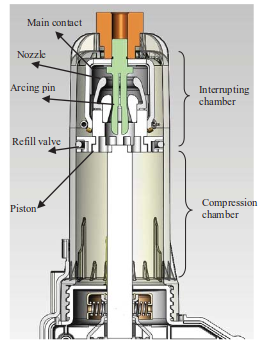
\includegraphics[scale=0.6]{Bilder/Theory/LBSselfblastandPuffer.png}
\caption{Schematic of a gas puffer interrupter \cite{bib:CBAC}.} \label{fig:selfBlastandPuffer}
\end{figure}

As can been seen in figure \ref{fig:selfBlastandPuffer}, the load break switch features many of the same components as a circuit breaker, but the dimensions are scaled down. The interruption technique used is puffer based, and the operation sequence is the same as illustrated in figure \ref{fig:CircutBreakPuff1}. The article "Gas flow analysis in low energy arc puffer interrupters" presents an experiment where the the pressure in the pressure chamber of a LBS is measured during opening operation, and is then is simulated, so that a comparison of the theoretical and measured pressures can be presented. In figure \ref{fig:airPressurePuffer}, the measured and simulated gas pressure from the paper are shown during a cold gas opening operation, which means that the switch was unloaded during the test. When certain loss factors have been included in the simulation, the simulation results corresponds quite well with the measured pressures.


\begin{figure} [H]
\centering
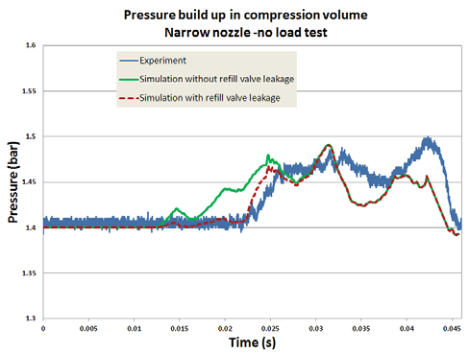
\includegraphics[scale=0.6]{Bilder/Theory/tankPressure.png}
\caption{Simulated pressure build up with different refill valve leakage settings compared to experimental results  \cite{bib:CBAC}.} \label{fig:airPressurePuffer}
\end{figure}

When introducing an arc to the system, the measured and simulated pressures change as shown in figure \ref{fig:airPressurePuffer2}. As seen in this figure, the pressure was not successfully simulated, and the difference between measured pressure and simulation results are huge, and increases with a longer arcing time. This simulation technique has been used with success when simulating for circuit breakers. This gives reason to believe that the properties of the arc alters significantly when the current is reduced, as in a load break switch. Good simulation tools for air flows when arcs like this are present are still to be developed, which makes scaling a circuit breaker down to an LBS without the possibility to know how the arc interacts with the gas flow difficult, especially when using air as interruption medium, and not SF$_6$.



\begin{figure} [H]
\centering
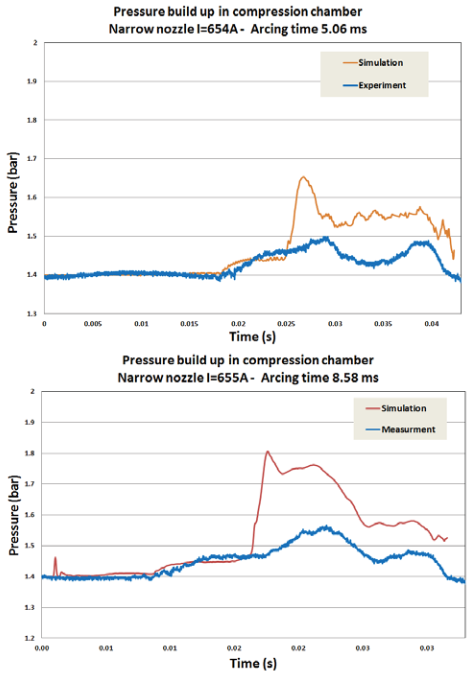
\includegraphics[scale=0.6]{Bilder/Theory/tankPressure2.png}
\caption{Pressure build up for load break tests with different arcing time   \cite{bib:CBAC}.} \label{fig:airPressurePuffer2}
\end{figure}

\subsection{Properties of the interrupting medium}
%As an interruption medium air is fairly good, and has been successfully used in the past to interrupt high currents at high voltages, some air-blast breakers are still in use. Dette hører kanskje inn i en innledning.
\subsubsection{Electrical conductivity in an arc} \label{sec:eleCondArc}
Gases have the ability to be good insulators as well as good conductors, mainly depending on the gas temperature. This is due to charged particles and electrons created by dissociation and ionisation of the molecules in the gas. Air is a mixture of several gases, but might be simplified to consist mostly of nitrogen (N$_2$). In figure \ref{fig:condAir}, the electrical conductivity of air as a function of temperature can be observed.

\begin{figure}[H]
\centering
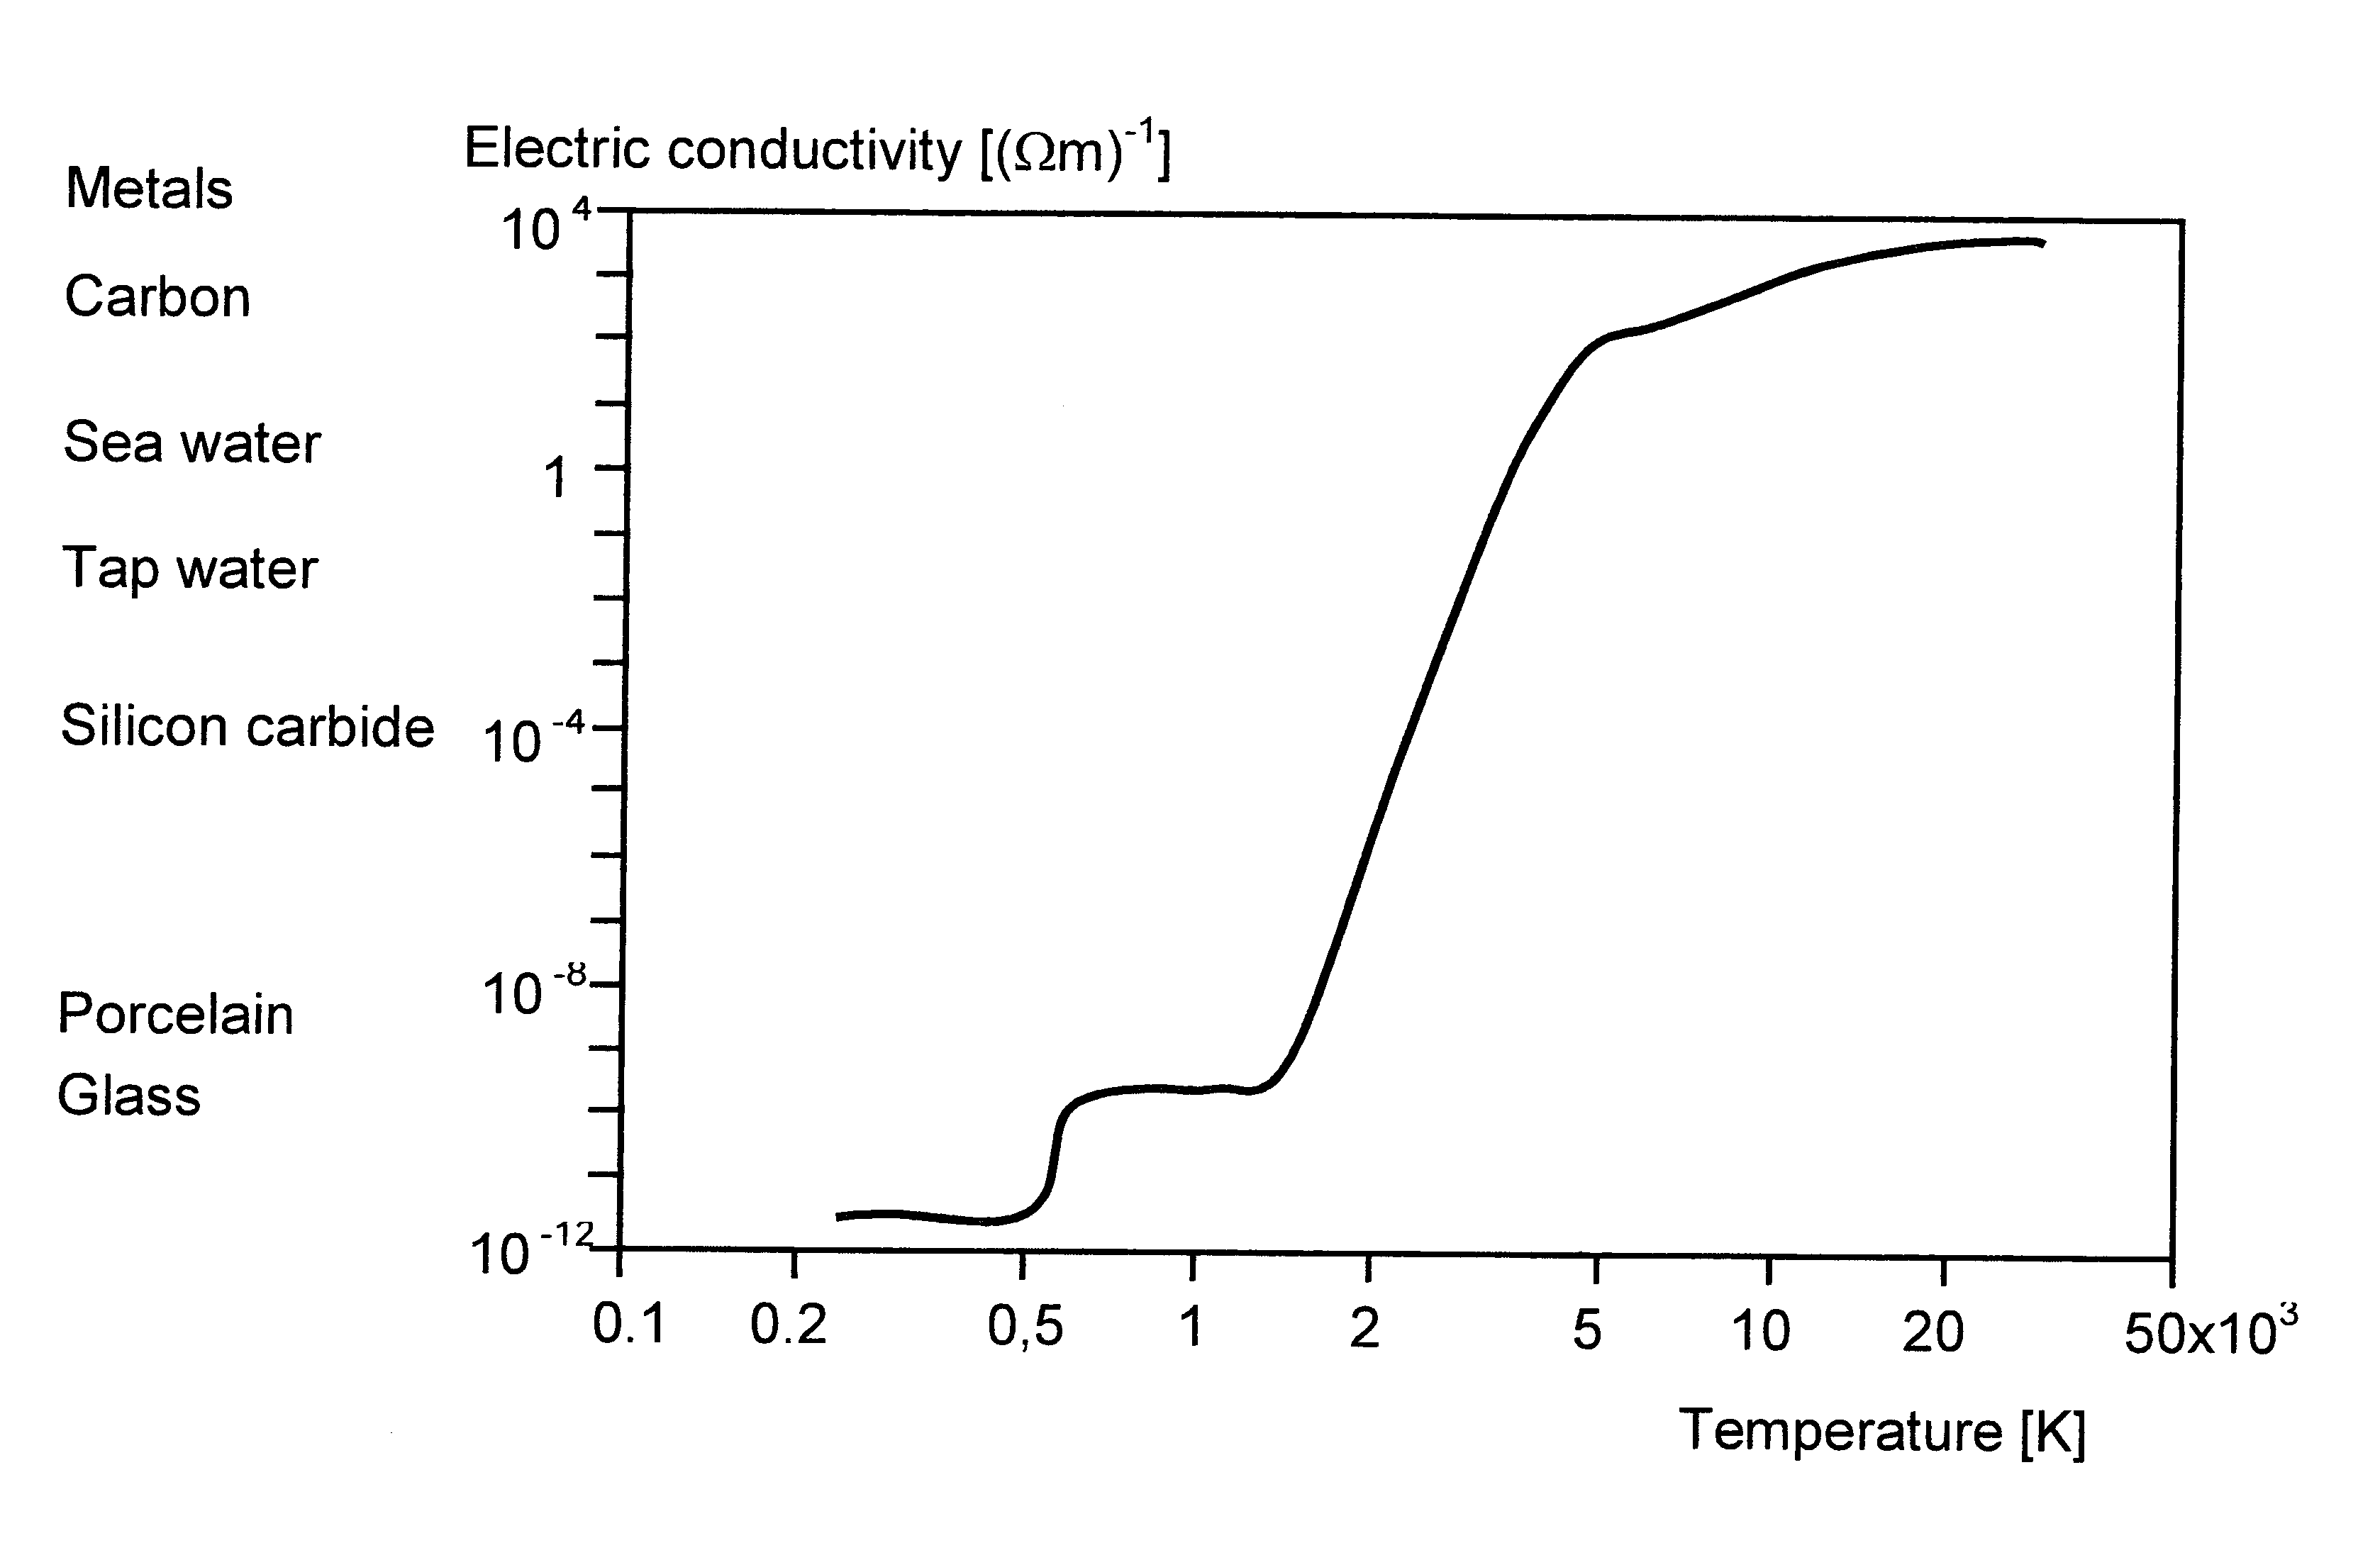
\includegraphics[scale=0.9]{Bilder/Theory/airConduct.png}
\caption{Electrical conductivity of air at atmospheric pressure \cite{bib:HVEbreak}.} \label{fig:condAir}
\end{figure}

The steep increase in conductivity can mainly be explained by the dissociation process and ionisation of N$_2$ due to temperature increase. The particle density of nitrogen as it dissociates due to high temperature in the gas is illustrated in figure \ref{fig:Ndensi}. When figure \ref{fig:Ndensi} is compared to figure \ref{fig:condAir}, a connection between temperature and the rapid decline of N$_2$, generation of the positive ion N$^+$, and the steep increase in conductivity of air is clearly presented.

\begin{figure}[H]
\centering
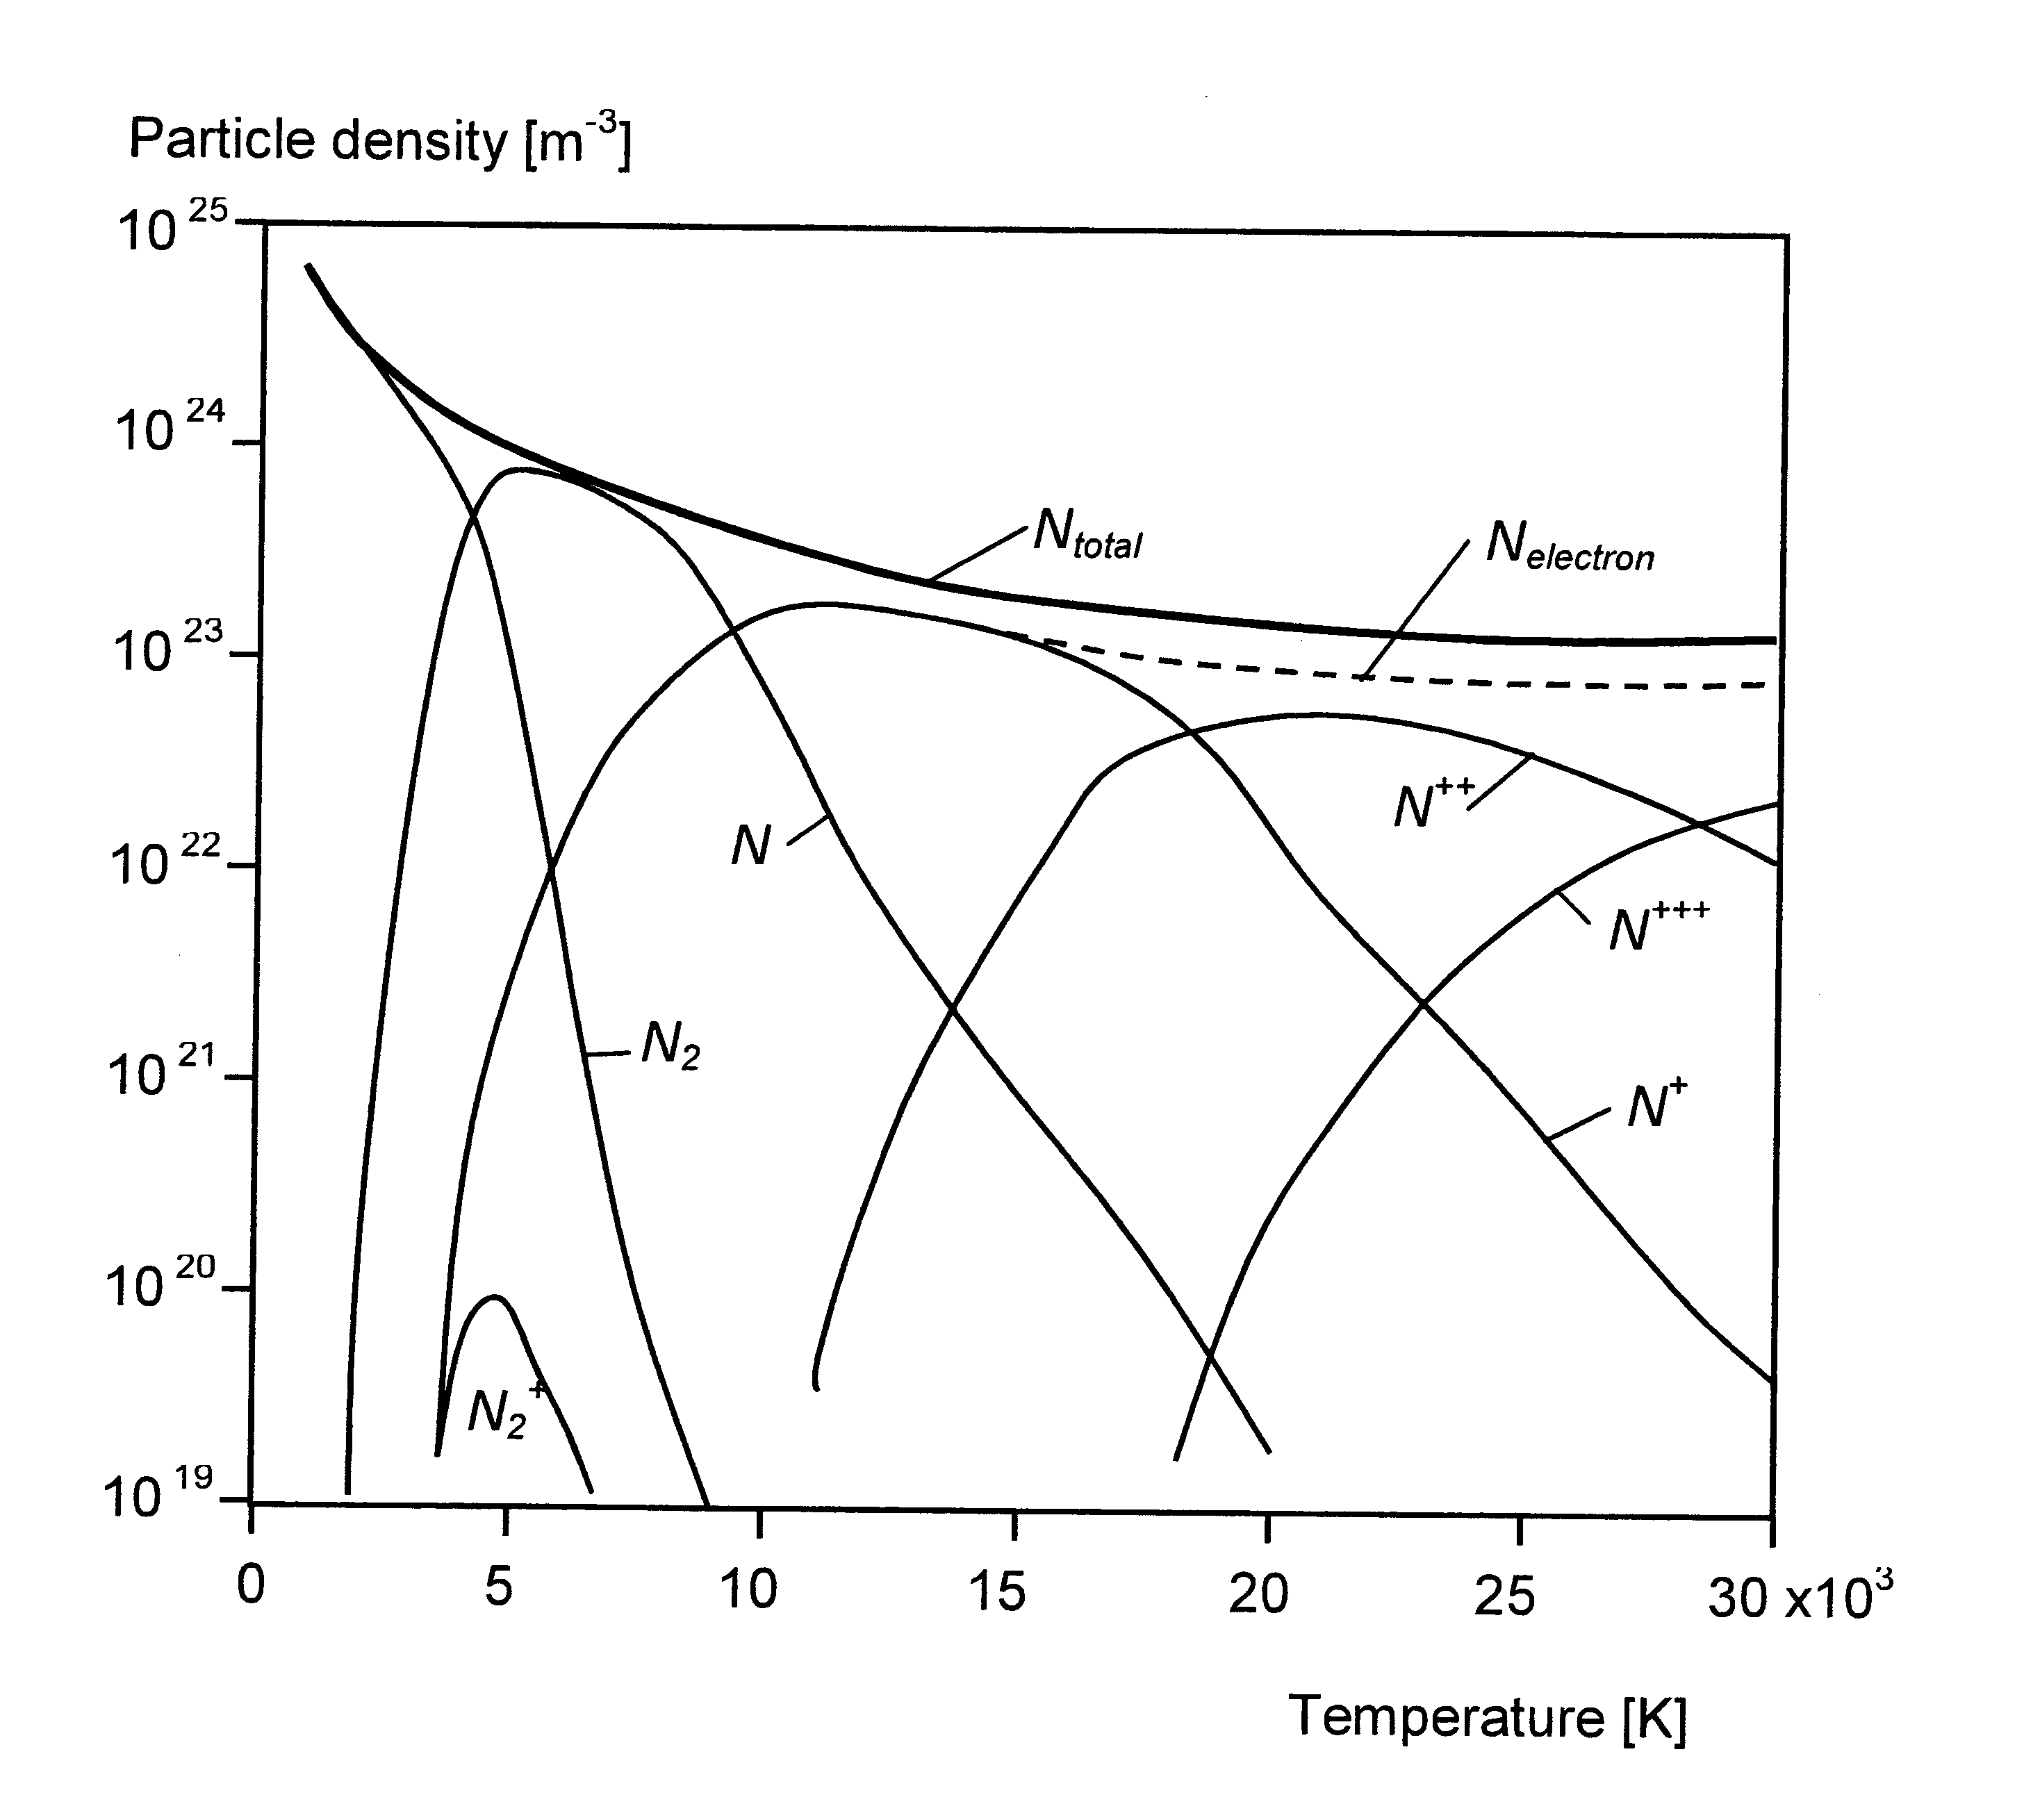
\includegraphics[scale=0.8]{Bilder/Theory/particleDensNit.png}
\caption{Particle density for different dissociation and ionisation products of nitrogen as a function of temperature \cite{bib:HVEbreak}.} \label{fig:Ndensi}
\end{figure}

Nitrogen is an electropositive gas, which means that it will have a tendency to give away electrons from its outer shell easily, especially when a strong electric field is applied and the gas is subjected to high temperatures. From figure \ref{fig:Ndensi}, the electropositive effect of N$_2$ is indicated via the generation of N$_{2}^{+}$ molecules. This reduces the breakdown voltage of the gas. From table \ref{tab:thermalIonisation}, the thermal ionisation energy for some gases is presented. This points out that N$_2$ has a significant lower ionisation energy than SF$_6$, and therefore gives away electrons more easily.

\begin{table}[H]
\center
\caption{Thermal ionisation energy for some gases \cite{bib:HVEbreak}.}
\begin{tabular}{|l|c|c|}
\hline 
Particle type & Single ionisation [eV] & Double ionisation [eV] \\ 
\hline 
Air & 16.3 &  \\ 
\hline 
N$_2$ & 15.8 &  \\ 
\hline 
N & 14.5 & 44.1 \\ 
\hline 
O$_2$ & 12.5 &  \\ 
\hline 
SF$_6$ & 19.3 &  \\ 
\hline 
S & 10.4 & 33.8 \\ 
\hline 
F & 17.4 &  \\ 
\hline 
\end{tabular} 
\label{tab:thermalIonisation}
\end{table}

During a interruption sequence, it is preferred to have different electrical conductivity of the interruption gas, depending on the current magnitude. When the current magnitude is high or raising, a good conductivity is needed. For most gases, including air, this is obtained because the gas is heated by the current travelling through it, resulting in a high temperature and a good conductivity. This is important for an interruption medium, as a low electrical resistance results in smaller losses, and therefore less heat generation of the surroundings. However, at the moment of CZ and after, a fast transaction from a conducting to an insulating state of the interruption gas is important, as this will avoid a re-ignition of the arc. At this stage, the interruption gas will use some time to recombine, due to both cooling and relatively slow movement of the particles the gas consists of. In addition to these effects, there will be free electrons in the contact gap, which increases the re-ignition chance. The oxygen in air is highly electronegative and will capture electrons. However, the concentration of oxygen is small relative to the concentration of nitrogen in air, and the electronegative effect is therefore weak. Because of this, a puffer is used to blow away the charged particles and hot gas between the electrodes to avoid a re-ignition.

\subsubsection{Heat transportation in an arc} \label{sec:HeatTransport}
There are several different thermal conductive mechanisms in an electrical arc. The effects of these mechanisms vary with temperature, and therefore the heat transport in the arc is strongly dependent upon the temperature. In figure \ref{fig:tempConGas}, the thermal conductivity of several common interrupting gases are compared as a function of temperature.

\begin{figure}[H]
\centering
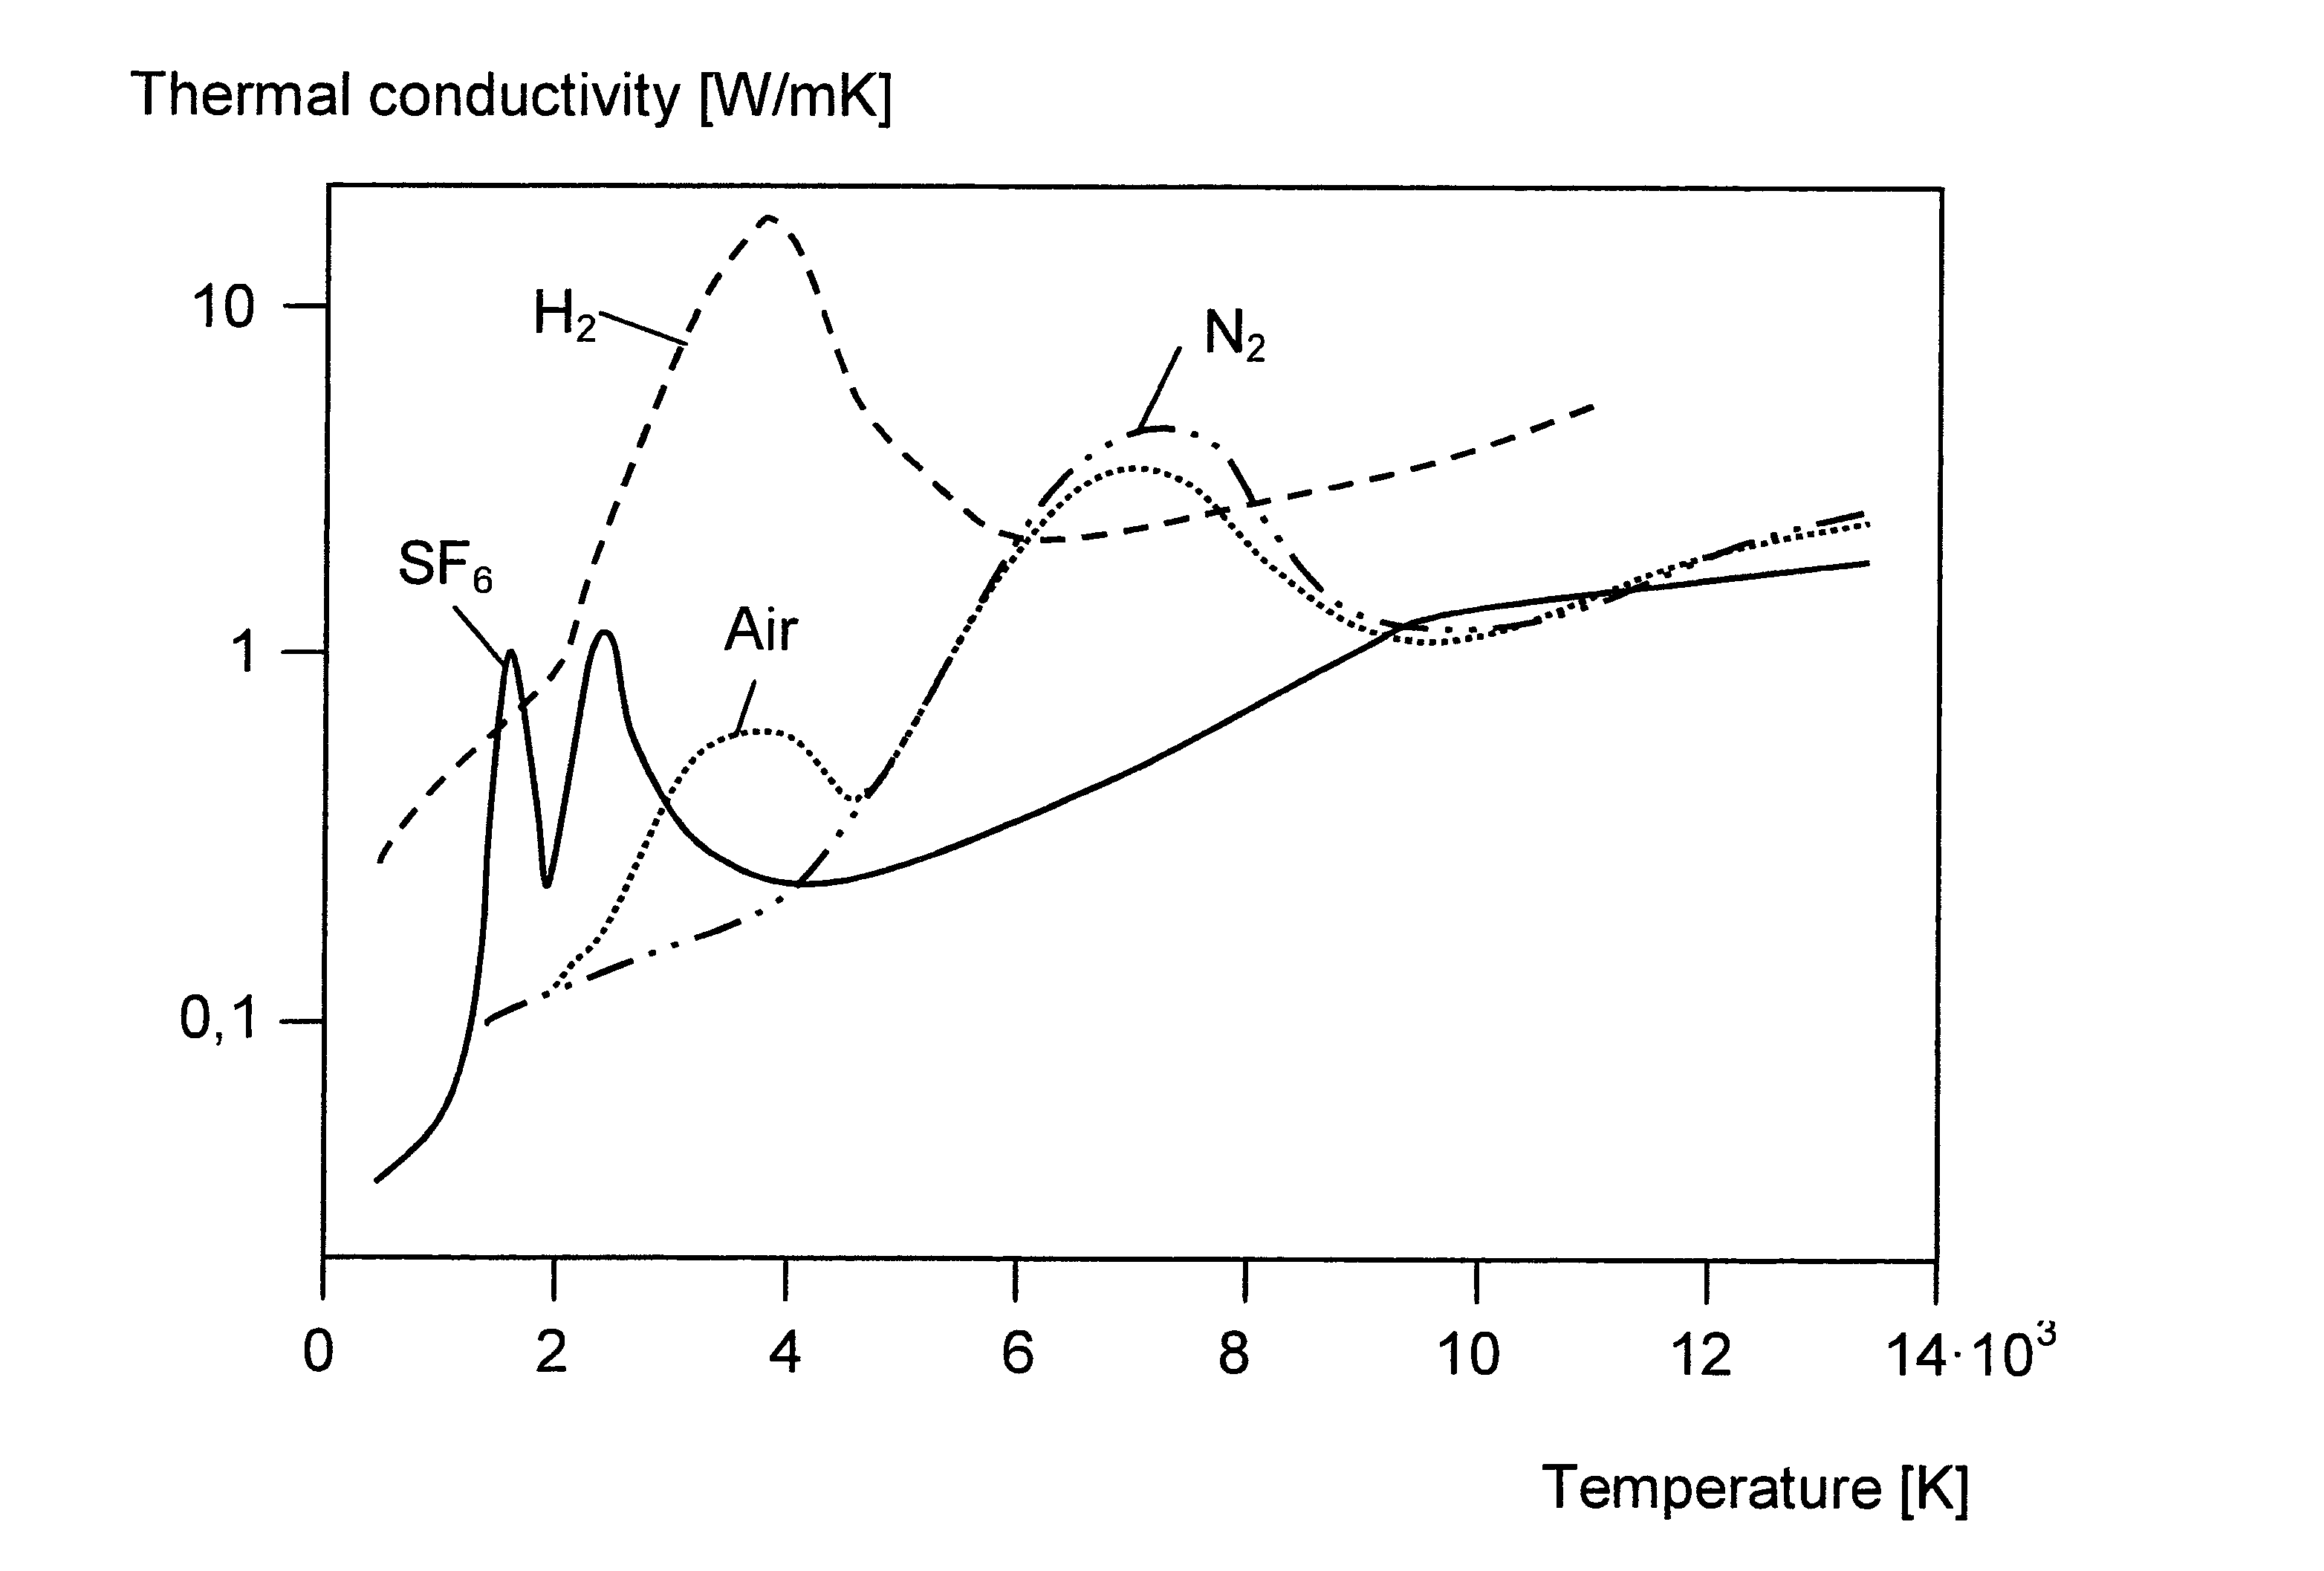
\includegraphics[scale=0.83]{Bilder/Theory/thermalCond.png}
\caption{Thermal conductivity for various gases as a function of temperature \cite{bib:HVEbreak}.} \label{fig:tempConGas}
\end{figure}

Due to the nature of the different stages in current interruption, it is desirable to use a gas that has a thermal conductivity that suits the different stages. When the current amplitude is rising, or is high, it is preferred that the thermal conductivity is low. This means that the plasma channel does not heat its surroundings, but mainly keeps the dissipated energy stored in its core. This will result in a temperature rise in the plasma channel and a relatively small increase in the surroundings. As explained in section \ref{sec:eleCondArc}, a high arc temperature will result in high conductivity in the arc, which gives a low arcing voltage. If the thermal conductivity is high in this region, more heating of the surrounding system will occur. This might result in a slower transaction between the conductive and insulating stage of the interrupting medium, due to the stored energy in the medium and the surroundings, resulting in a higher chance of re-ignition.

At the moment right before CZ, it is an advantage if the thermal conductivity of the gas is high. This will result in a fast cool-down time of the plasma channel, since both the current amplitude is decreasing and the energy stored in the arc now is released to its surroundings. A gas with high thermal conductivity in this stage of the interruption process will be able to recombine from an ionised and highly conductive to a non-conductive state fast, making it more difficult for a thermal re-ignition to occur. This is because of the quick cooling of the plasma channel. In gases where the thermal conductivity is low, the cooling mechanisms are of great importance, since a quick recombination of ionised gas does not occur in the same manner as when the medium is quickly cooled. Therefore, removal of hot gas and charge carriers must be done differently. This is described in detail in section \ref{sec:genDes}. The thermal conductivity profile of air is not well suited for current interruptions, at least compared to the one of SF$_6$. If figure \ref{fig:tempConGas} is consulted, it can be observed that air has a high conductivity when the temperature is high, and a low conductivity when the temperature is low. This is the opposite of the preferred characteristics. Even though air has a small peak in thermal conductivity between 3000 K and 4000 K, its thermal conductivity profile is regarded as one of the major challenges when using air as an interruption gas. 

The temperature distribution in a plasma channel can be divided into three sections \cite{bib:TDCIGBB}, as illustrated with figure \ref{fig:tempDist1}. Zone 1 is the highly conductive arc core and also the zone with the highest temperature. Zone 2 acts as an energy buffer during the decay of the arc, while zone 3 is the cold gas surrounding the arc. When using cooling-mechanisms to quench the arc, it is primarily the second zone of the temperature profile that is cooled. The first zone's temperature will mainly be dependent on the current passing through the arc, and will not be influenced by the cooling mechanism in the same degree. If the cooling is sufficient, the energy stored in zone 2 when the arc approaches CZ is low, and therefore its effect as an energy buffer is reduced, resulting in a rapid decline in temperature in the arc core as the current approaches zero. This makes the interrupting medium's ability to transport energy important when investigating efficient cooling methods. As figure \ref{fig:tempConGas} has pointed out, SF$_6$ has the ability to transfer heat between zone 1 and 2 fast in the correct temperature range compared to the interrupting sequence. Air has to a lesser degree the ability to do this.

\begin{figure}[H]
\centering
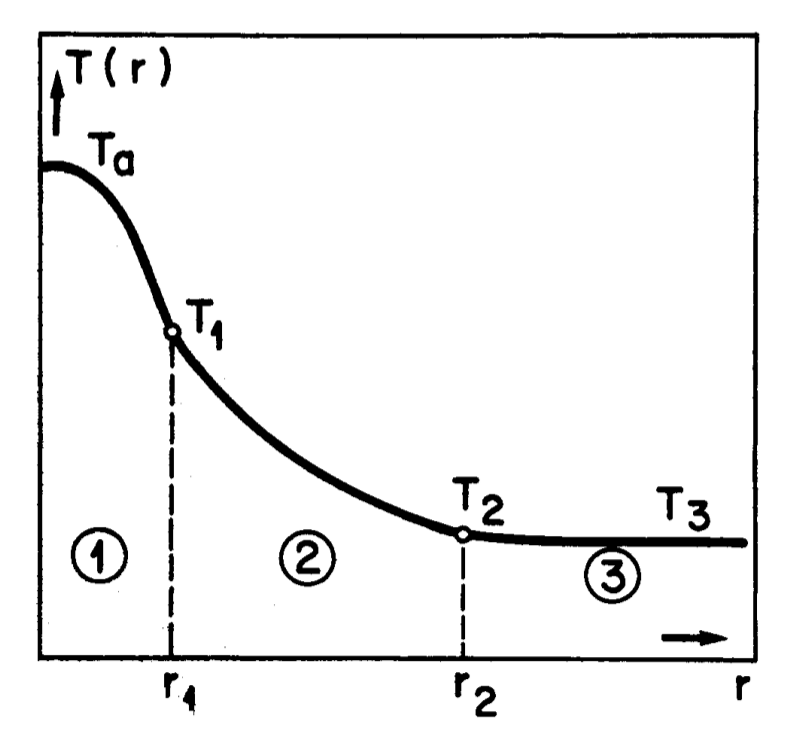
\includegraphics[scale=0.25]{Bilder/Theory/tempZonesArc.png}
\caption{Radial temperature distribution in a plasma channel \cite{bib:TDCIGBB}.} \label{fig:tempDist1}
\end{figure}

Figure \ref{fig:tempDist2} shows how the temperature distribution varies with the electrical current. Due to radiation losses in the arc, the temperature has an upper limit of about 20 000 K to 30 000 K. At this point the cross-section of the arc will increase, rather than the temperature. However, it is not common for an LBS to experience these temperature ranges, and its temperature distribution will mainly be in the lower current ranges in figure \ref{fig:tempDist2}.

\begin{figure}[H]
\centering
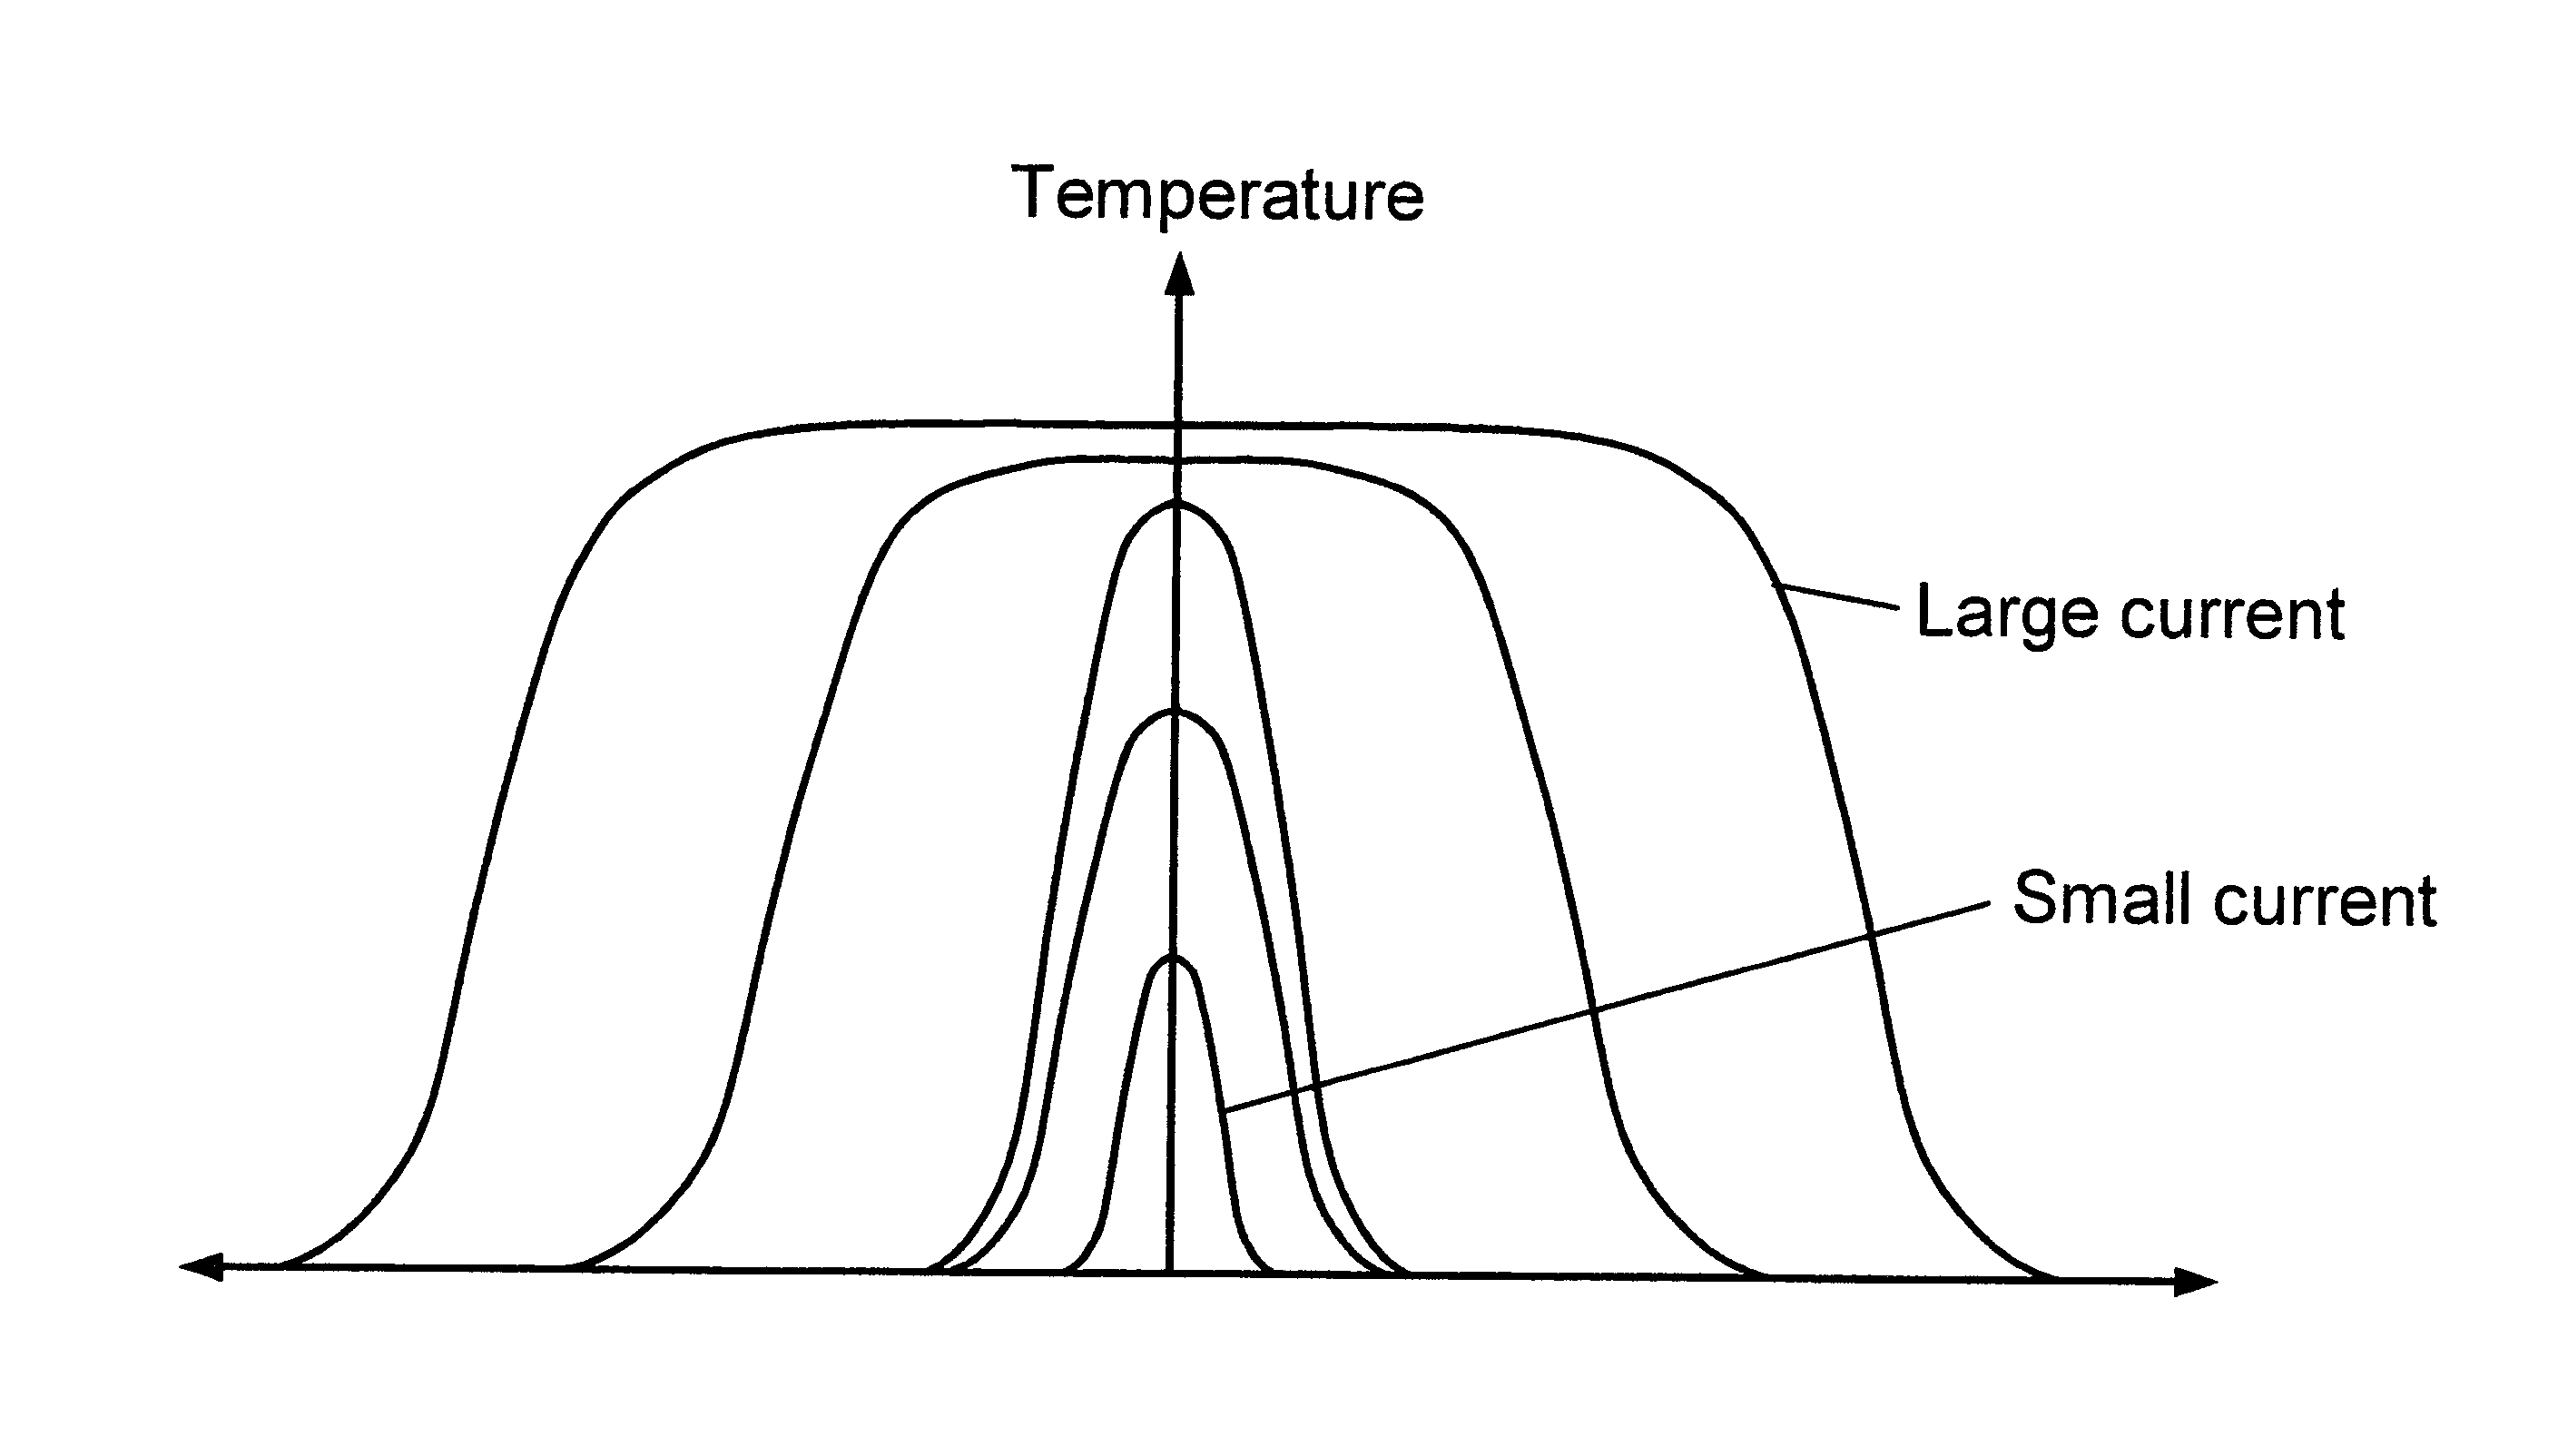
\includegraphics[scale=0.85]{Bilder/Theory/plasmaChannel1.png}
\caption{The radial temperature distribution in a plasma channel for different current magnitudes \cite{bib:HVEbreak}.} \label{fig:tempDist2}
\end{figure}

\subsection{Arcing voltage}
Most of the information in section \ref{sec:genDes} is collected from \textit{"Current Interruption in Power Grids"} by Magne Runde \cite{bib:HVEbreak} \newline

\subsubsection{Static arcing voltage}
It is common to distinguish an arc into two different types. The most common is called a dynamic arc, the other a static arc. A static arc can only be established when using DC current, and after any transients have died out. Therefore, static arcs are uncommon, and in nearly all switching operations the properties of the arc is best described by the dynamic arc model.

AC currents always generate a dynamic arc. This is because the current alters with time, and thereby the properties of the arc. In cases where DC current is used, but external factors like cooling varies over time, like in a puffer based switchgear, the arc is dynamic. When dealing with AC switchgear with a puffer based interruption method, the arc is always a dynamic arc. Due to the complexity of a dynamic arc, it is common to regard the arc to behave like a static arc within a certain time interval, and therefore some properties of a static arc will be described in this section. Dynamic arcs will be featured further in section \ref{sec:dynARC}.

The static arc characteristic is illustrated in figure \ref{fig:staticArcChar}. This describes the relationship between current and arcing voltage in a static arc. The scaling of the axes is only approximate and may vary with gas type and electrode material.

\begin{figure}[H]
\centering
\includegraphics[scale=1]{Bilder/Theory/staticArcChar.png}
\caption{Static arc characteristic  \cite{bib:HVEbreak}.} \label{fig:staticArcChar}
\end{figure}

As can be seen from figure \ref{fig:staticArcChar}, the characteristic is highly non-linear. At low currents, like tens of amperes, the voltage drop across the arc decreases with increasing current. Then the voltage is constant, and apparently independent from the current flowing in the arc. How large, and in which current range, the constant part of the arcing voltage occurs depends highly on what gas the arc burns in. For currents above this range, the arcing voltage starts to increase with the current.

In figure \ref{fig:potDisArc} the potential distribution of an electrical arc is illustrated. A static electrical arc might be regarded as divided into three regions:

\begin{description}
\item[Cathode region:] The voltage drop, $\mathrm{V_c}$, is usually around 20 V.
\item[Arc column:]	There is a constant electric field in this region, typical 1 V/mm.
\item[Anode region:] The voltage drop, $\mathrm{V_a}$, is usually around 3 V.
\end{description}

\begin{figure}[H]
\centering
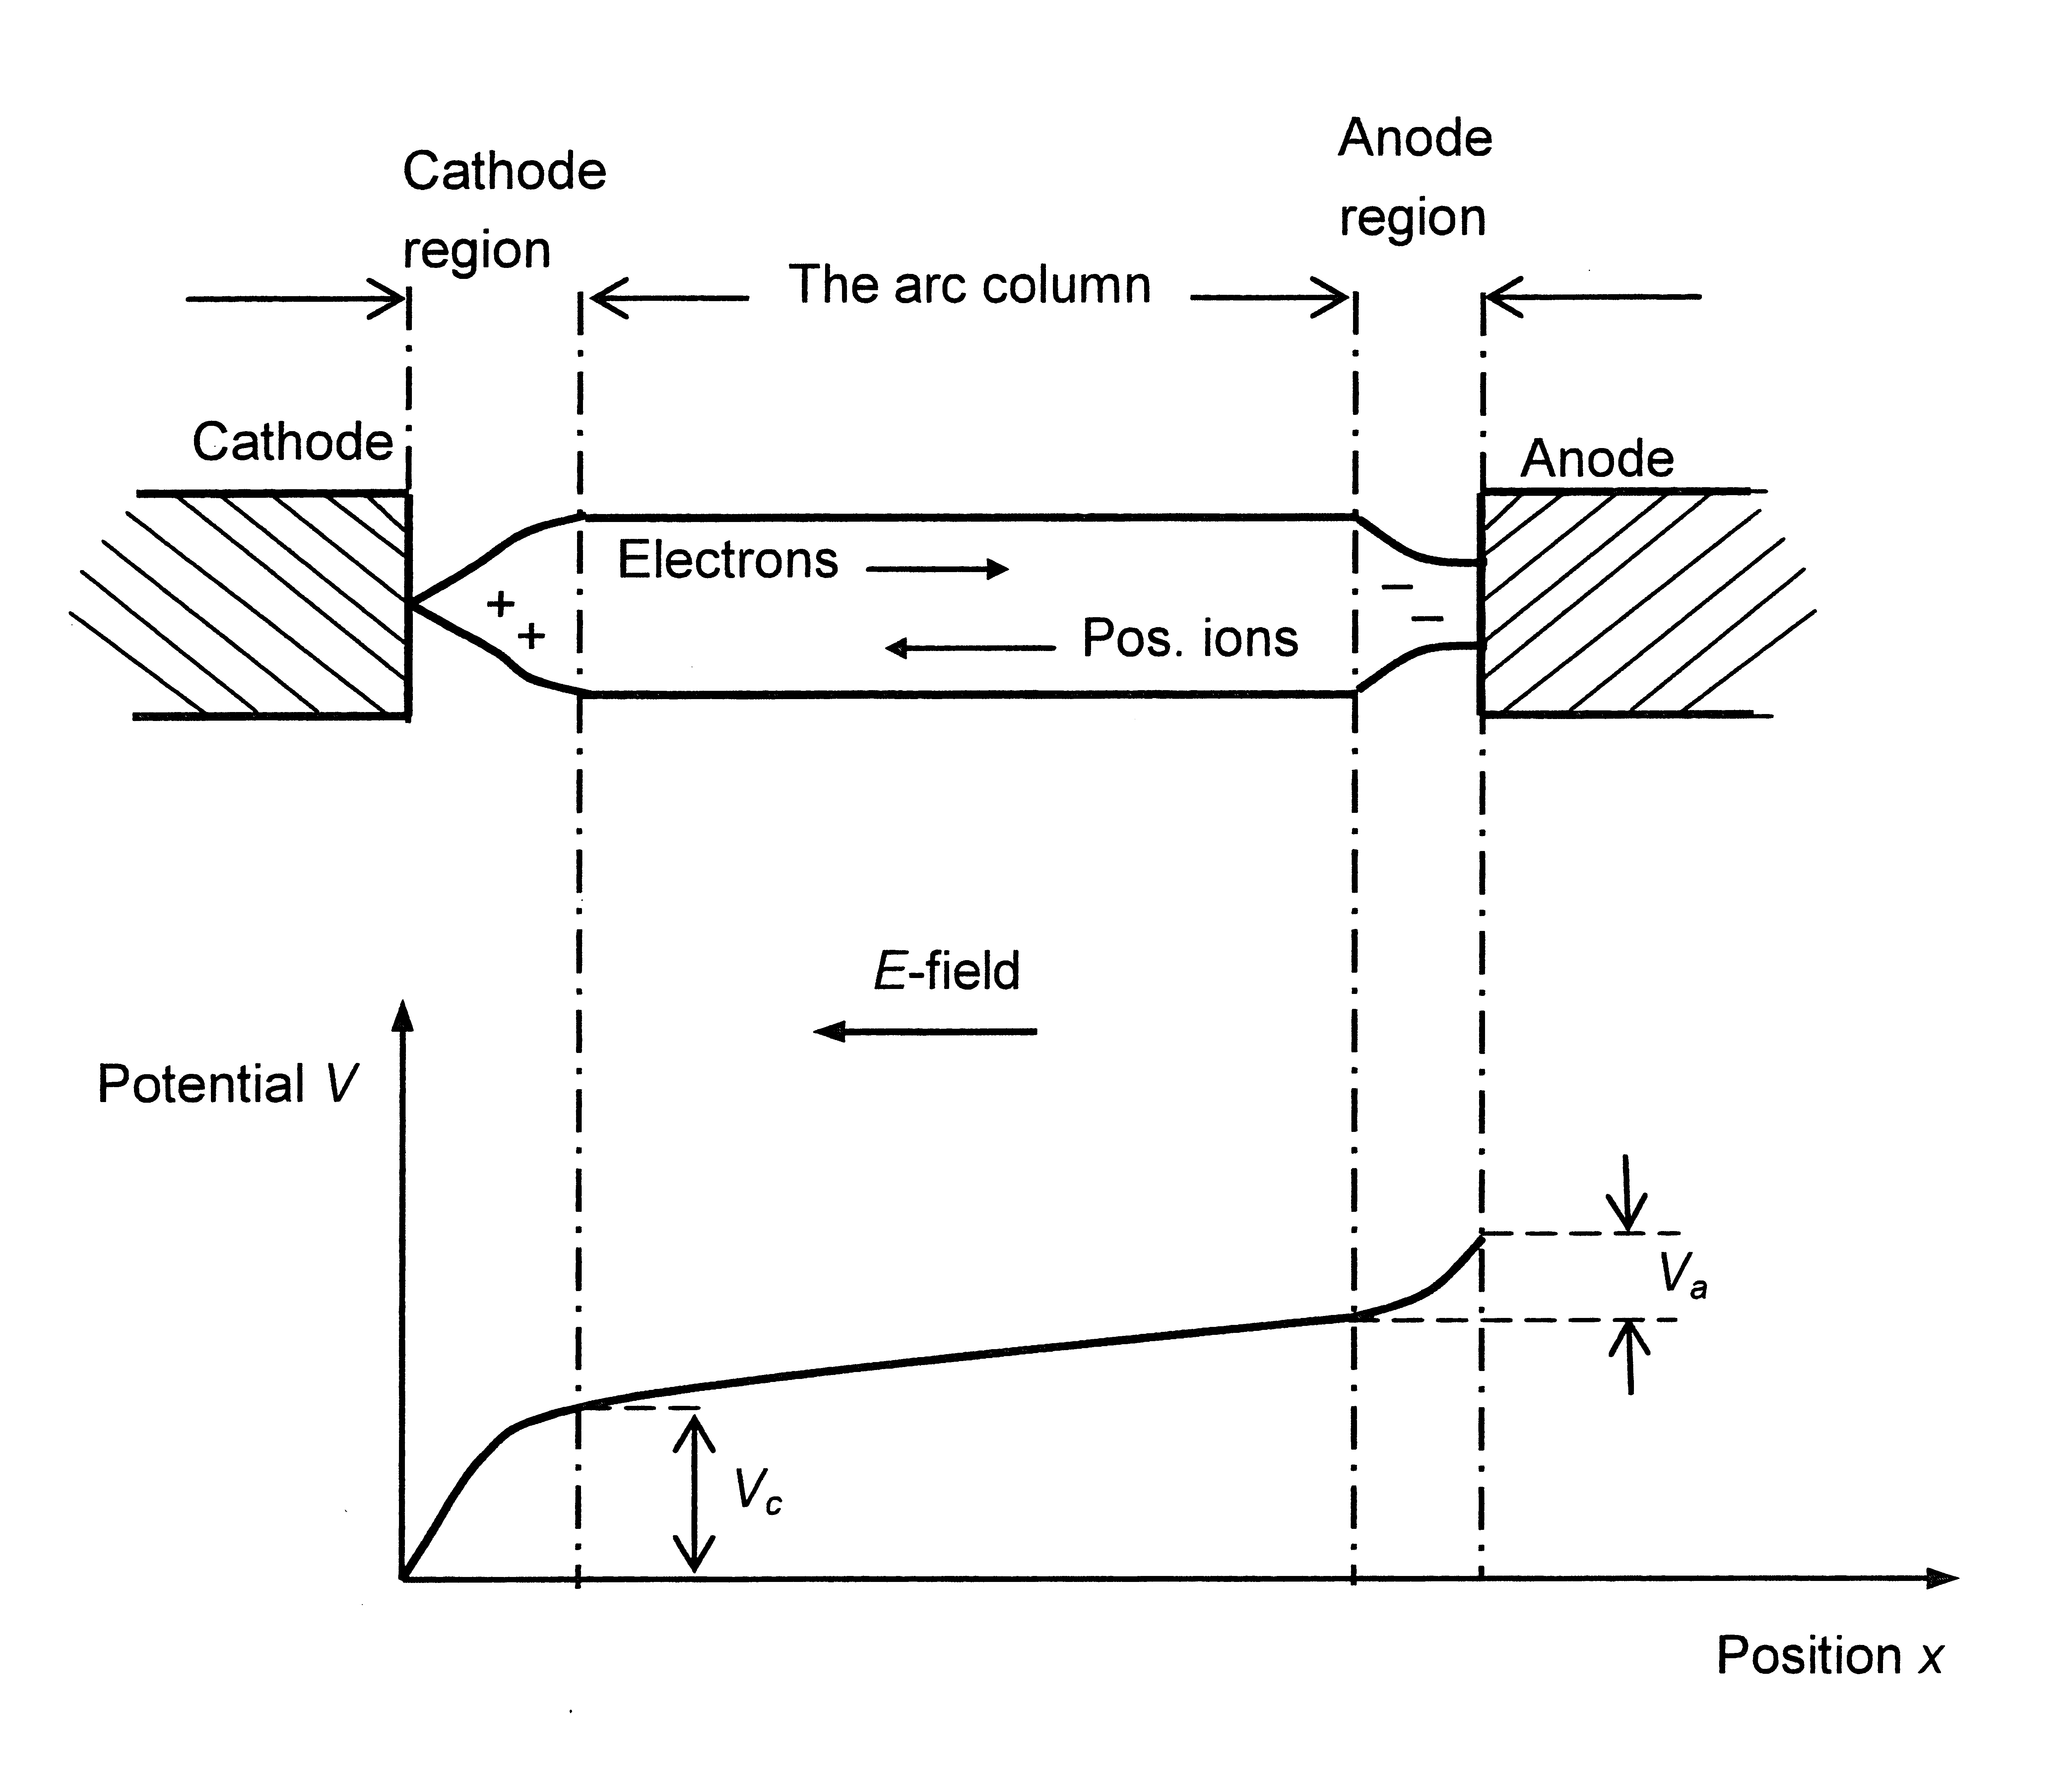
\includegraphics[scale=0.8]{Bilder/Theory/potentialDistArc.png}
\caption{Cross-section of a stationary arc and the corresponding potential distribution \cite{bib:HVEbreak}.} \label{fig:potDisArc}
\end{figure}

The description above is highly general, and the voltage distribution will vary depending on which gas the arc is burning in, as well as the current range and the electrode materials being used. Therefore, the potential distribution across a dynamic arc that burns in air for a typical current range of an LBS is analysed. The analyse is based on results from previously conducted tests performed with the test circuit presented in section \ref{sec:testCir}.

Three interruption test, where a thermal re-ignition occurred after the first CZ and the second CZ, are selected. The pressure in the pressure chamber was held constant throughout the whole test, and was set to 1.0 bar upstream pressure. The RMS value of the current was 630 A, while the contact and nozzle geometry was the same for each of the three tests. In figure \ref{fig:threeTests}, the arcing voltage during the three chosen interruption tests is shown.

\begin{figure}[H]
\centering
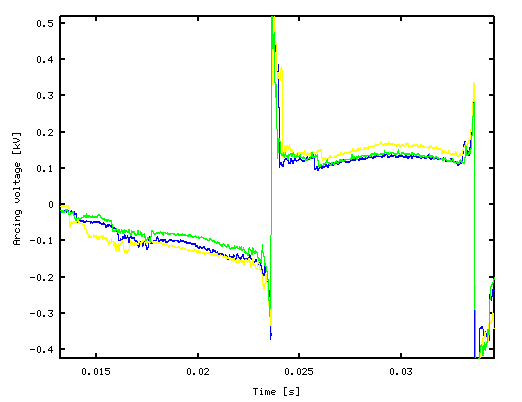
\includegraphics[scale=0.7]{Bilder/Theory/threeTests.png}
\caption{Arcing voltage during three interruption tests. The y-axis is arcing voltage in kV and the x-axis is time in seconds from test start.} \label{fig:threeTests}
\end{figure}

The average arcing voltage from these three tests is presented in figure \ref{fig:averageArcingVoltage}, and it is applied to approximate the potential distribution of the burning arc.

\begin{figure}[H]
\centering
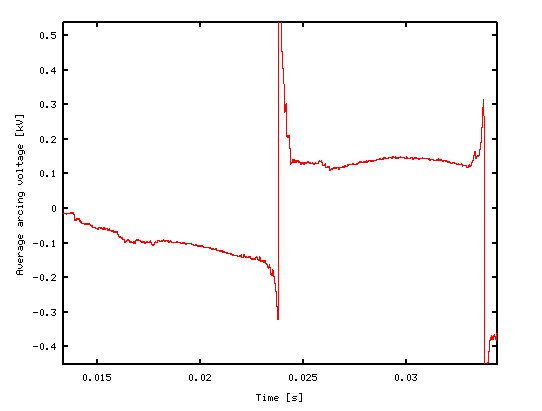
\includegraphics[scale=0.7]{Bilder/Theory/averageOfthreeTests.png}
\caption{Average arcing voltage for three interruption tests. The y-axis is arcing voltage in kV and the x-axis is time in seconds from test start.} \label{fig:averageArcingVoltage}
\end{figure}

In both figure \ref{fig:threeTests} and \ref{fig:averageArcingVoltage}, contact separation occurs at $t \approx 0.0140$ s. The first CZ occurs at $t \approx 0.0235$ and the second CZ occurs at $t \approx 0.0335$ s. The arcing time, the time from contact separation to the first CZ, is approximately 9.5 ms for all the three tests.

The length of the arc is determined by the distance between the contacts, which moves apart with a constant speed of approximately 5 m$/$s. When the length of the arc is short, most of the arcing voltage will be close to the electrodes. To establish an estimate over the voltage drop in close vicinity of the electrodes, the average voltage when the contacts were between 0.4 mm and 1.4 mm apart was calculated. Because of transients in the arcing voltage when the arc ignites, a contact gap length less than 0.4 mm was unsuited for this use. Due to the short length of the arc in this time span, the average arcing voltage in this region can represent an approximation of the voltage drop close to the electrodes. This voltage drop is estimated to 33 volts in absolute value, when using the procedure above.

Then the increase in arcing voltage per millimetre is calculated. Linear regression when the arc is between 23.2 mm and 38.8 mm is used to establish the rate of rise in the arcing voltage, and thereby the increase in arcing voltage caused by elongation of the arc can be established. This rate of rise was calculated to be 2.7 V$/$mm in absolute value.

The final expression in absolute value for the voltage across the arc, where x is the length of the arc in millimetres, then becomes:
\begin{equation}
V(x) \approx 2.7x+33 \ \ \ \ x \in [0.4, 40.0] \ \mathrm{mm}
\end{equation}

This estimation of the arcing voltage fits well in the region between contact separation and the first CZ. In the region between first and second CZ, this model is not suited. It is assumed that the values calculated here will be dependent on both upstream pressure and test current.


\subsubsection{Dynamic arcing voltage} \label{sec:dynARC}
When the current, or cooling of the arc changes with time, the arcing voltage no longer follows the static arc characteristics presented in figure \ref{fig:staticArcChar}. This is because the temperature cannot change instantaneously, since it is impossible to use an infinite amount of power to heat or cool a certain mass instantaneously. This gives an arc a certain thermal inertia. During a short time span, cooling can be regarded as constant, while the current is set by the input power.

Thermal inertia causes the arc to "remember" the amplitude of the current that just has passed for a short time. If the current follows a step function, the arc voltage will at first take a higher value, and then gradually decrease to the value corresponding to the static arc characteristic, as presented in figure \ref{fig:timeConstantStep}. This is because the arcing voltage mainly is set by the electrical conductivity of the arc, which is highly dependent on the temperature. Since the temperature cannot change instantaneously, the arcing voltage can be regarded as a function of time with an exponential decay. The time constant of this decay varies from gas to gas. In table \ref{tab:timeConstants}, the time constant for some gases is displayed. The time constant for each gas depends on several factors, like test method and current magnitude. The variation of the time constant alters with the current, and can to a certain degree be compared to the inverse of the thermal conductivity's dependency of temperature presented in figure \ref{fig:tempConGas}, where the temperature is proportional to the current. 

\begin{figure}[H]
\centering
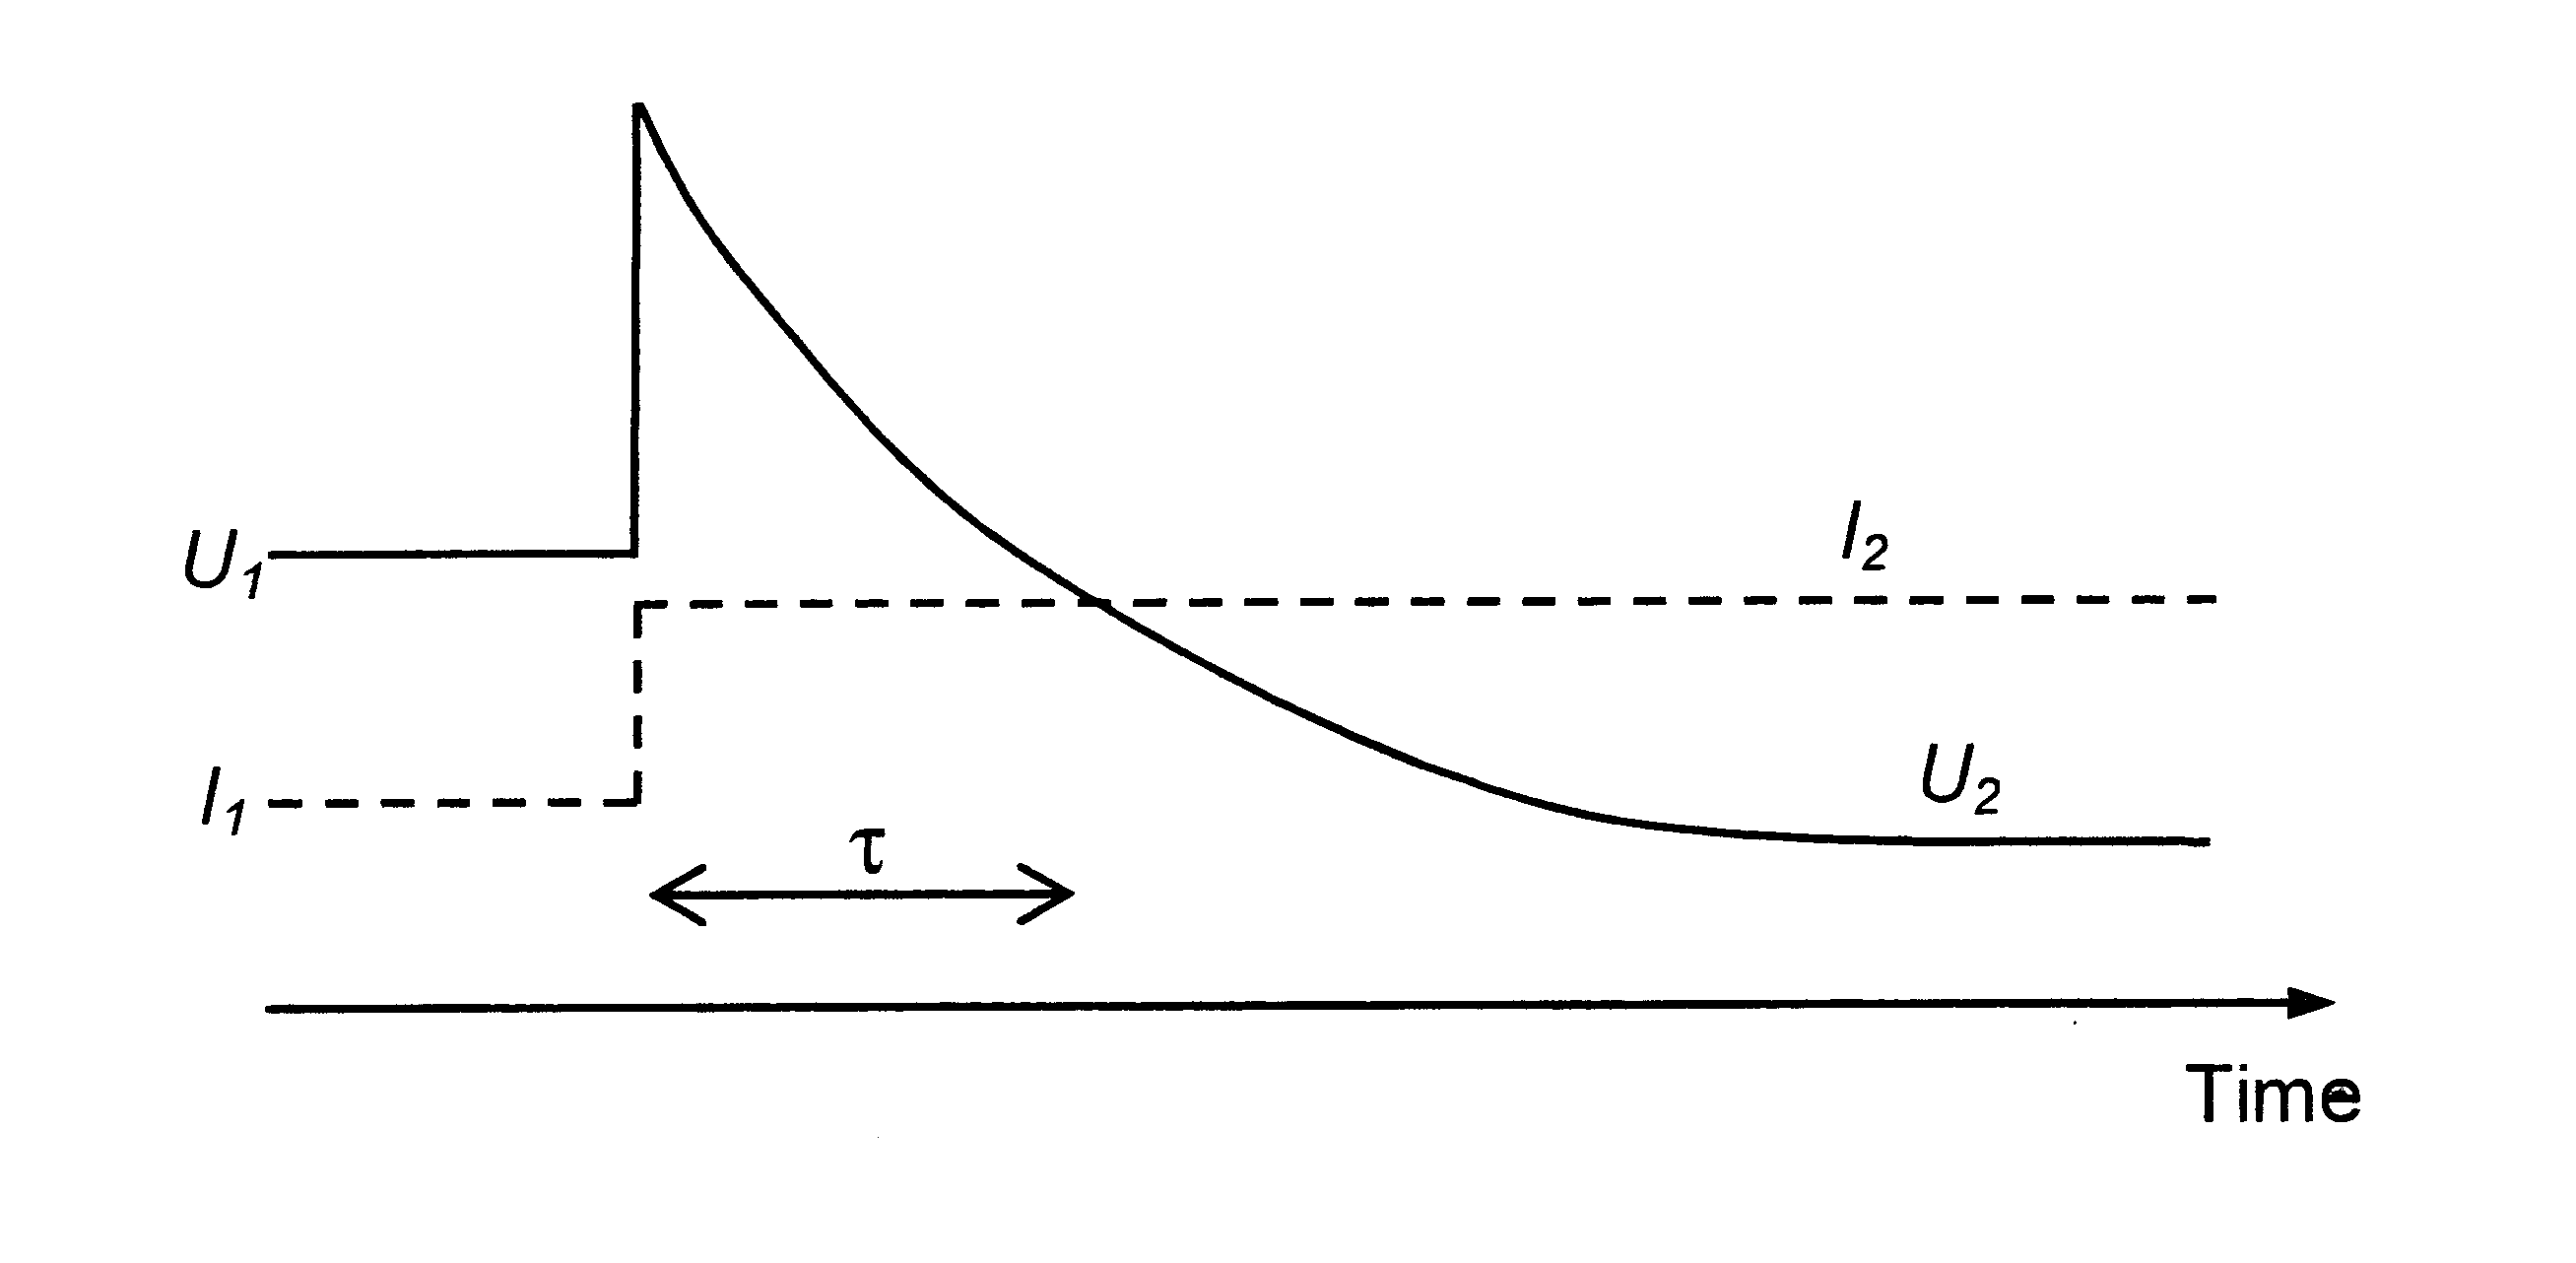
\includegraphics[scale=1]{Bilder/Theory/timeConstants.png}
\caption{Voltage drop of an arc exposed to a current that follows a step function  \cite{bib:HVEbreak}.} \label{fig:timeConstantStep}
\end{figure}

\begin{table}[H]
\center
\caption{Time constants in a 1 A arc burning in a 19 mm tube \cite{bib:HVEbreak}. }
\begin{tabular}{|c|c|}
\hline 
Gas & Time constant [$\mu$s] \\ 
\hline 
SF$_6$ & 0.8 \\ 
\hline
O$_2$ & 1.5 \\
\hline
CO$_2$ & 15 \\
\hline
Air & 80 \\
\hline
N$_2$ & 210 \\
\hline
H$_2$ & 1 \\
\hline
\end{tabular} 
\label{tab:timeConstants}
\end{table}

A gas with a low time constant is faster to cool, and thereby reduces its electric conductivity faster than a gas with a high time constant. This is an advantage during current interruption. Air has a fairly high time constant resulting in a slower cool-down time than other interrupting gases. This is closely related to the problems mentioned in section \ref{sec:HeatTransport}. 

In figure \ref{fig:arcingVoltageFre}, the arcing voltage for a dynamic arc is illustrated. As shown by the figure, the arcing voltage varies both with current and frequency. In figure \ref{fig:arcingVoltageVSCurrent}, the arcing voltage with regard to current for a previously conducted interruption test is shown. As can be observed from this figure, the arcing voltage follows the same pattern as an dynamic arc burning at 50 Hz shown in figure \ref{fig:arcingVoltageFre}. Some differences in the burning conditions for the arc in figure \ref{fig:arcingVoltageFre} and \ref{fig:arcingVoltageVSCurrent} are present. In figure \ref{fig:arcingVoltageFre}, the arc is not cooled and the contacts are stationary with a fixed gap. In figure \ref{fig:arcingVoltageVSCurrent}, the arc is cooled with a 1.0 bar upstream pressure, while elongated by the separation of the contacts.

\begin{figure}[H]
\centering
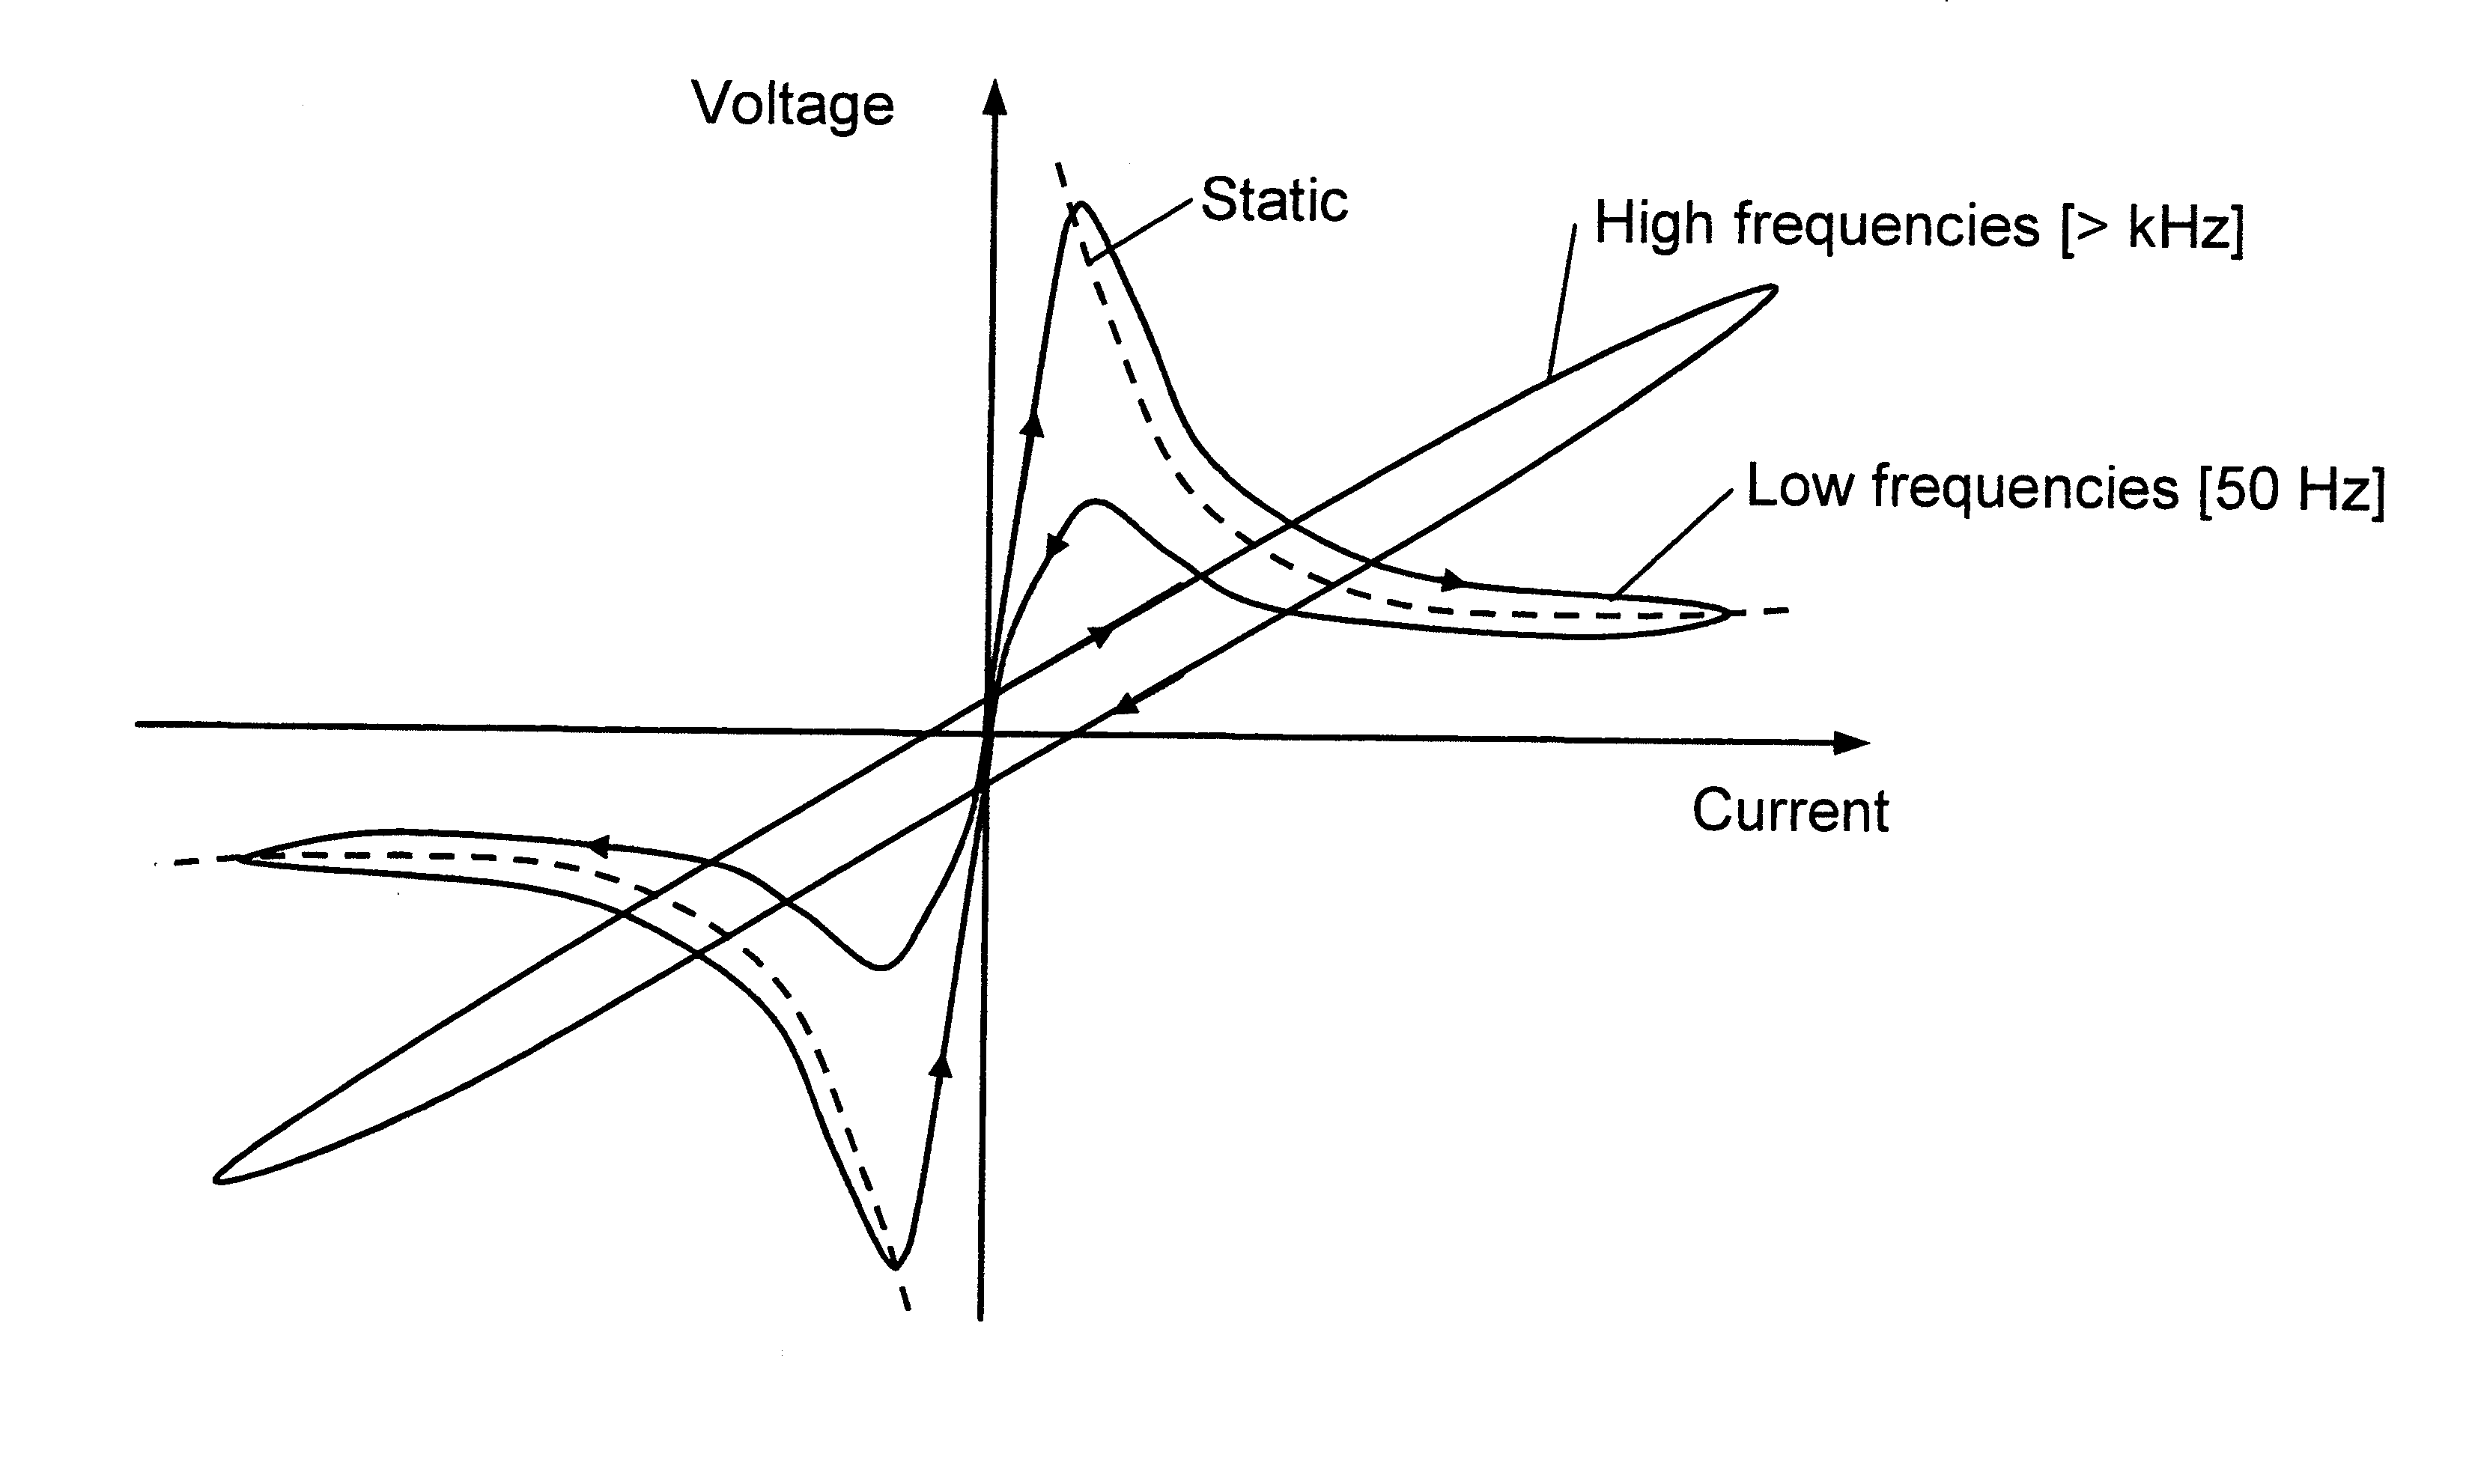
\includegraphics[scale=1]{Bilder/Theory/dynamicArcingVoltage.png}
\caption{Static, low, and high frequency arc characteristic  \cite{bib:HVEbreak}.} \label{fig:arcingVoltageFre}
\end{figure}

\begin{figure}[H]
\centering
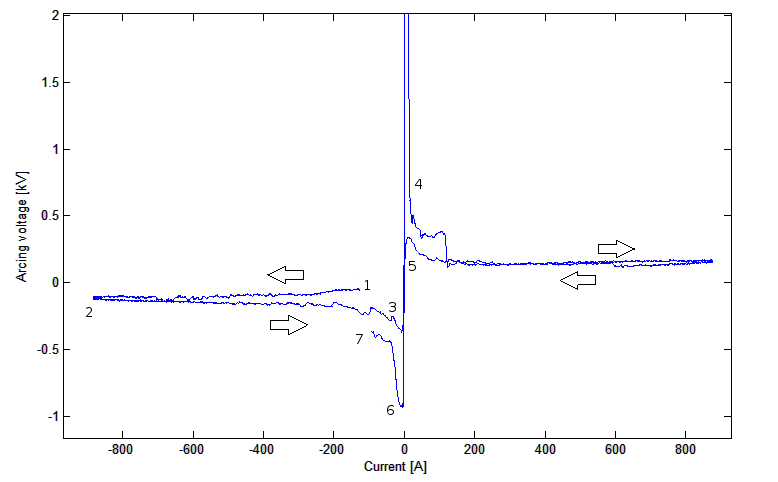
\includegraphics[scale=0.7]{Bilder/Theory/arcingVoltagevzCurrent3.png}
\caption{Arcing voltage during a full power cycle in a test interruption.} \label{fig:arcingVoltageVSCurrent}
\end{figure}

The numbered parts in figure \ref{fig:arcingVoltageVSCurrent} represents different aspects of the arc during the interruption sequence, and are described in the list below. The arrows represent the direction of time during the interruption. A full power cycle is plotted in the figure, resulting in a time span of 0.02 seconds.
\begin{description}
\item[1:] The contacts separate and the arc ignites. As the absolute value of the current increases, the arcing voltage follows the same trend as illustrated in figure \ref{fig:arcingVoltageFre}.  
\item[2:] After the first current peak, the arcing voltage is always higher than than the corresponding arcing voltage for the same current magnitude that occurred before the current peak.
\item[3:] The arcing voltage increases as the current decreases, then at the moment of the first CZ, the arc is quenched and a high voltage peak arises.
\item[4:] Quickly after CZ, a thermal re-ignition occurs and the arc re-ignites. The high voltage peak that occurred during CZ is probably due to the intensive cooling the arc experiences. Some distortion of the arc causes the arcing voltage to drop and the pattern seen in figure \ref{fig:arcingVoltageFre} is disturbed, but the same trend can be observed.
\item[5:] The arcing voltage rises as the second CZ approaches.
\item[6:] Almost instantly after CZ, the arc reforms as a thermal re-ignition occurs.
\item[7:] Mainly due to elongation of the arc, the arcing voltage is higher at this point than in the beginning (point 1). If the length of the arc had remained constant throughout the whole experiment, the arcing voltage would be expected to be approximately the same at point 7 and point 1. The arc has now burnt a full power cycle, t=0.02 s, from ignition.
\end{description}

\subsection{Thermal re-ignition considerations}
As mentioned in section \ref{sec:puffer} the main purpose of the puffer mechanism is to remove charge carriers between the contacts after CZ to avoid re-ignition of the arc. After CZ a strong electrical field rises between the electrodes, represented by the recovery voltage. This electrical field will accelerate the charge carriers in the air-gap, and the movement of these will represent a current called the post-arc current (PAC). During a high current, high voltage interruption for a circuit breaker, the peak of the PAC is usually a few amperes or less, and have a duration for some microseconds. For currents and voltages in the LBS range the current peak of the PAC is expected to be considerably smaller.

A thermal re-ignition is avoided if the PAC has reached zero, since this means that the charge carriers in the air-gap is gone. On the other side, a thermal re-ignition occurs if the PAC rises, an arc ignites, and the current obtains its common sinuous form. Figure \ref{fig:PACbreakandreIgnite} shows the PAC for a successful and an unsuccessful interruption. 

\begin{figure} [H]
\centering
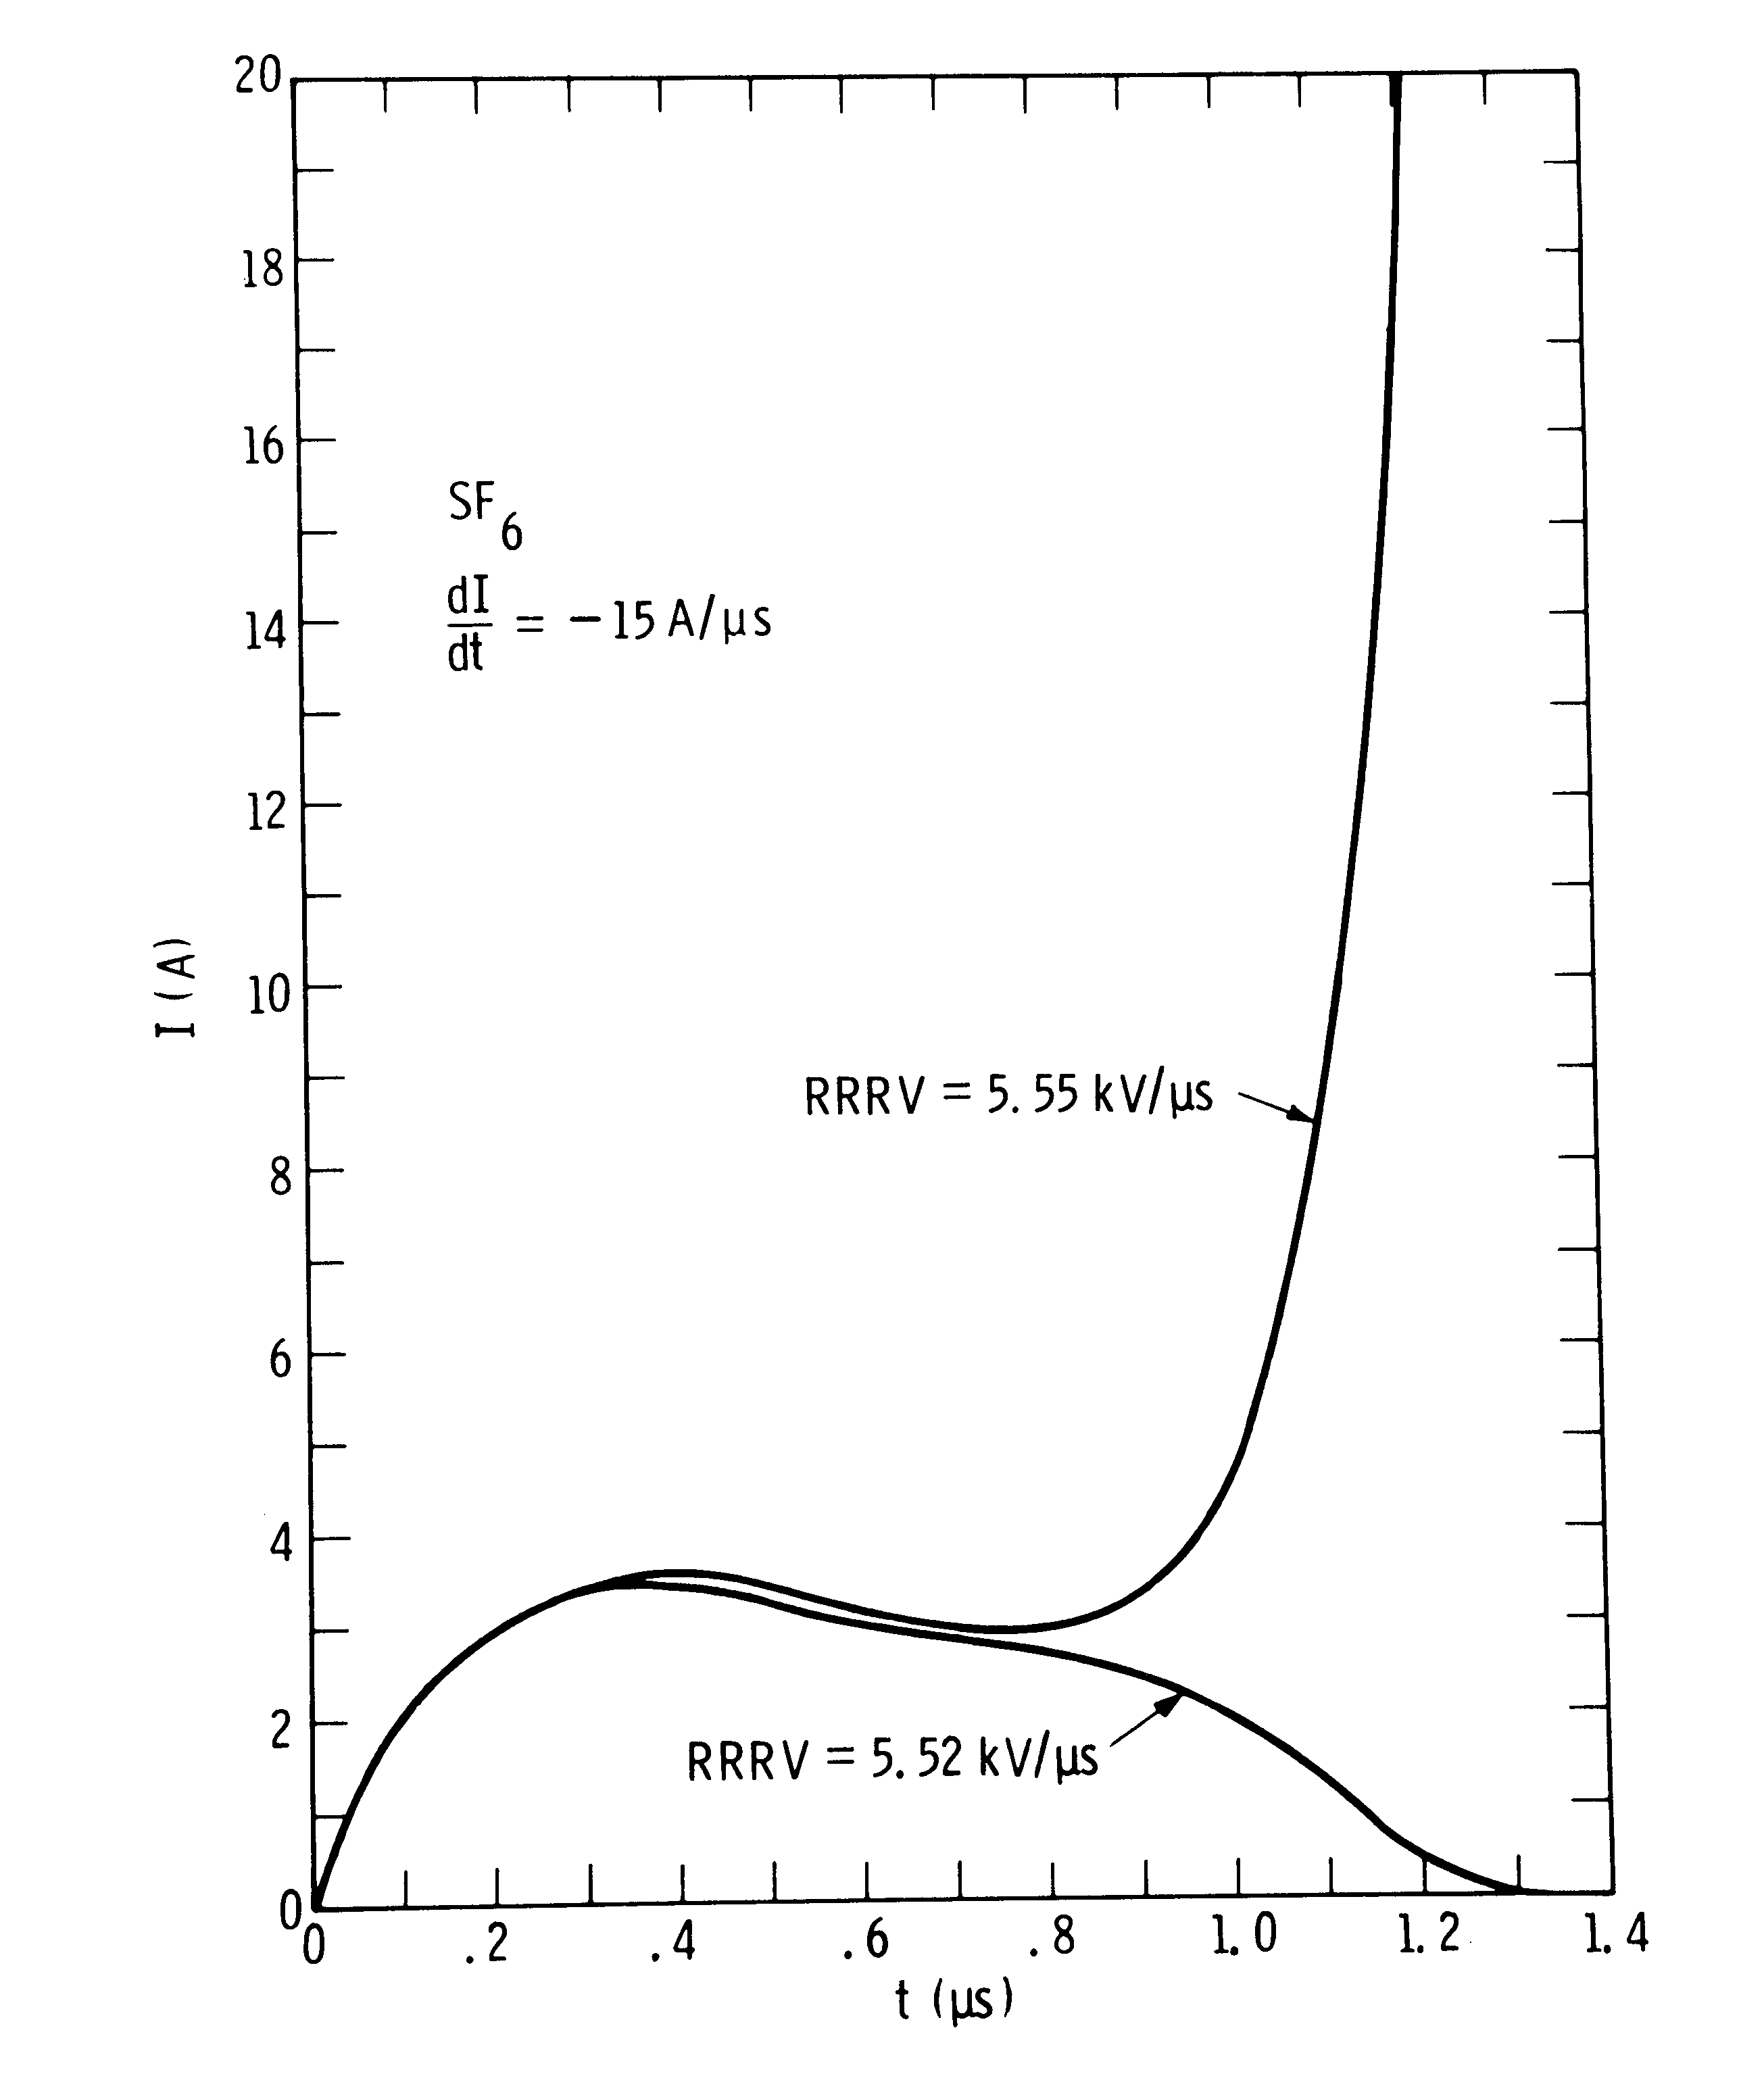
\includegraphics[scale=0.7]{Bilder/Theory/failSuccPAC.png}
\caption{The post-arc current during a successful and unsuccessful interruption \cite{bib:CIHVN}.} \label{fig:PACbreakandreIgnite}
\end{figure}

The thermal interruption success rate is partly determined by the amount of stored energy in the arc and in its surroundings. Power is the product of arcing voltage and current. The energy produced by the arc is the integral (the area under the power as an function of time graph) of the power during a certain time span. Research has shown that only the energy dissipated close to CZ have an effect on the interruption capabilities and that the cooling from the air flow mainly effects the interruption rate between 50 to 100 microseconds before CZ \cite{bib:CIHVN}.

The parameter $\delta \mathrm{I}/\delta \mathrm{t}$ can be used to describe the energy losses close to CZ. In figure \ref{fig:freqComp} two currents with the same $\delta \mathrm{I}/\delta \mathrm{t}$ close to CZ can be observed.

\begin{figure} [H]
\centering
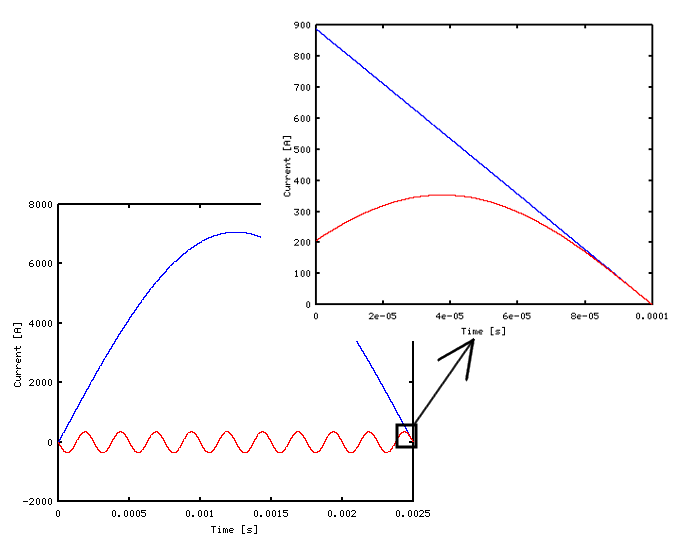
\includegraphics[scale=0.6]{Bilder/Theory/diffFreq3.png}
\caption{Comparison of $\delta \mathrm{I}/\delta \mathrm{t}$ for a 200 Hz and 4000 Hz current wave.} \label{fig:freqComp}
\end{figure}

These two currents, even though with completely different frequency and amplitude have proven almost equally difficult to interrupt \cite{bib:CIHVN}. Therefore, it is assumed that the effect of a puffer is most efficient close to CZ where the energy dissipation is almost equal and right after CZ when the PAC is present. The graph in the lower part of the picture in figure \ref{fig:freqComp} shows the a half period of the 200 Hz current besides several periods of the 4000 Hz current, while the upper part of the figure shows both currents 100 $\mu$s before CZ. As can be seen form the figure $\delta \mathrm{I}/\delta \mathrm{t}$ for the 200 Hz and the 4000 Hz current is almost alike for the last 50 $\mu$s before CZ.

The thermal inertia of the interruption gas, as described with the time constants presented in table \ref{tab:timeConstants} gives a relation over how fast the PAC is reduced. Gases with a long time constant will probably have a longer time span for the PAC. Air has a fairly large time constant and problems with thermal re-ignitions can partially be explained by this.

As described in this section the thermal re-ignition chance will depend on several factors. The $\delta \mathrm{I}/\delta \mathrm{t}$ close to CZ will give an estimate over the energy dissipation in the arc and the temperature in the plasma. This will both influence the current peak and time of the PAC. The time constant of the interruption gas gives an indication over how fast the gas responds to changes from for example cooling. A long time constant might lead to slower cooling of the arc, resulting in a higher amplitude and time span of the PAC. The steepness of the recovery voltage is also important as a fast increase in this voltage will accelerate the charge carriers that makes up the PAC, resulting in a larger re-ignition chance. Further information on this topic can be collected from the book: "Current Interruption In High-Voltage Networks".


\subsection{Air flow considerations}
During the interruption process, a puffer based switch uses a piston to drive an air flow to quench the arc. The energy losses from the arc is transported away by this air flow as described in section \ref{sec:HeatTransport}. The efficiency of the cooling depends on the speed and mass of the air flow, as well as how the flow is guided on the arc. In figure \ref{fig:airPressurePuffer2}, a typical pressure development in the pressure chamber of an LBS is illustrated during interruption. However, in the test switch presented in section \ref{sec:testSwitchandContact} and used in the interruption tests conducted in this report, the pressure is more or less constant throughout the whole interruption process. This is because it uses a large pressure reservoir rather than a piston to drive the air flow.

The mass flow ,$\dot{m}$, of air through the nozzle can in most interruption cases be regarded as conserved, and is presented in equation \eqref{eq:massFlow}. The mass density ,$\rho$, depends on pressure and temperature, while the volume flow ,\textit{Q}, depends on speed and area, as presented in equation \eqref{eq:volumeFlow}.

\begin{equation} \label{eq:massFlow}
\dot{m}=\rho Q
\end{equation} 

\begin{equation} \label{eq:volumeFlow}
Q=\int v \ dA
\end{equation}

In equation \eqref{eq:volumeFlow}, the area ,\textit{A}, if considering the volume flow rate in a nozzle is the cross-section area of the nozzle. This will vary depending on where in the nozzle the volume flow is calculated, as well as the arcing contact's position. The speed of the air flow ,$v$, depends on the pressure difference ,$\Delta p$, between the pressure chamber and the interruption chamber, and it will increase with an increasing pressure difference. An increase in air flow velocity will result in a greater mass flow, which if guided properly will lead to a more efficient cooling of the arc. In the test switch used during the experiments conducted in this report the efficiency of the cooling can be set by adjusting the pressure in the pressure reservoir before interruption as described in section \ref{sec:testCir}.

\cleardoublepage
\section{Method}

\subsection{Test circuit} \label{sec:testCir}

Figure \ref{fig:testSwitchRiggEq} illustrates the physical appearance of the test switch. The numbered parts are: 1. Compressed air reservoir (connected to the high voltage supply circuit), 2. Tulip contact, 3. Nozzle, 4. Pin contact, 5. Connection to load circuit, 6. Spring drive mechanism, 7. Electromagnet release mechanism, and 8. Position transducer.

\begin{figure} [H]
\centering
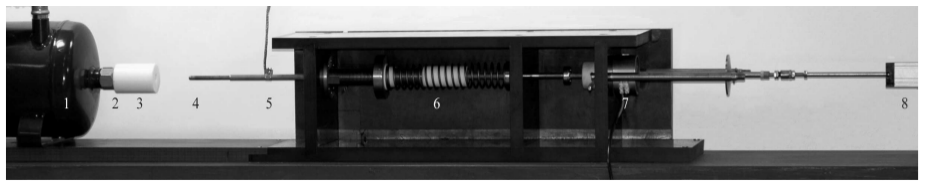
\includegraphics[scale=0.4]{Bilder/Method/switchTest.png}
\caption{The physical appearance of the test switch \cite{bib:AFIMVLBA}.} \label{fig:testSwitchRiggEq}
\end{figure}

Figure \ref{fig:testCurcuit} displays the laboratory test circuit used for the interruption tests. The circuit is designed to supply a 50 Hz / 13.8 kV current. It is possible to shape the transient recovery voltage (TRV) by tuning the parameters L$_1$, L$_s$, R$_1$, R$_d$, and C. The systems' short circuit parameters are R$_{sc}$ and L$_{sc}$. The TRV generated during interruption is set to simulate the standard for a 24 kV / 630 A class from the International Electrotechnical Commission (IEC), which corresponds to:

\begin{itemize}
\item The initial part of the TRV has a rate of rise in recovery voltage (RRRV) of 71 - 73 V / $\mu$s.
	\begin{itemize}
		\item The voltage difference is measured over the first 20 $\mu$s after CZ.
	\end{itemize}
\item The first voltage peak is between 7.0 and 7.4 kV, with a rise time of approximately 96 $\mu$s.
\end{itemize}

\begin{figure} [H]
\centering
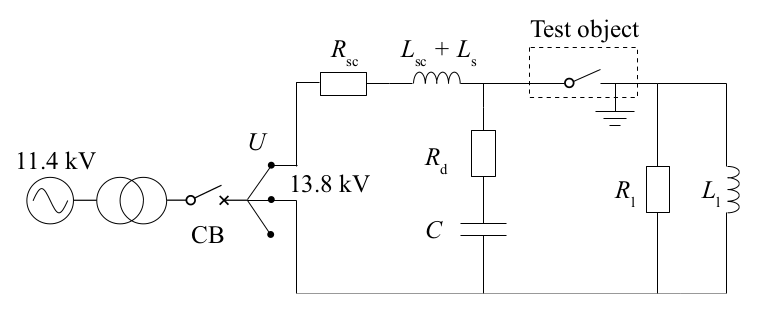
\includegraphics[scale=0.35]{Bilder/Method/circuit.png}
\caption{Circuit used for the interruption test \cite{bib:AFIMVLBA}.} \label{fig:testCurcuit}
\end{figure}

In table \ref{tab:testParameters}, the values of the different test circuit parameters and the corresponding currents can be observed. The test is conducted at currents with an RMS value of 630 A and 880 A. In the entire experiment, the TRV is kept constant up to and including the first voltage peak. In the case of a failed interruption, a thermal re-ignition occurs within a few microseconds after CZ.

\begin{table}[H]
\center
\caption{Circuit parameters and resulting currents \cite{bib:AFIMVLBA}. }
\begin{tabular}{|c|c|c|c|c|c|}
\hline 
L$_s$ [mH] & L$_1$ [mH] & R$_1$ [$\Omega$] & C [nF] & R$_{d}$ [$\Omega$] & I [A] \\ 
\hline 
6.9 & 86.2 & 22.1 & 102 & 198 & 630 \\ 
\hline
2.9 & 60.2 & 15.1 & 156 & 170 & 880 \\
\hline   
\end{tabular} 
\label{tab:testParameters}
\end{table}

A resistive transducer is measuring the contact position, while a Hall Effect current transducer is measuring the current through the test switch. The voltage between the contacts is measured with a parallel resistive / capacitive voltage divider. All measurements are transmitted through optical fibres to a 12 bit resolution transient recorder with a sampling frequency of 2.5 MHz. The pressure in the tank is only measured before each test with an accuracy of 0.01 bar. A "Cheetah 1470", a near-infrared (NIR) high-speed camera, records the opening sequence of the switch and the arc that burns between the contacts with a frame rate of ?? fps.

\subsection{The switch and contact geometry} \label{sec:testSwitchandContact}
This experiment is conducted using copper-tungsten arcing contacts, polytetraflourelthylene (PTFE) nozzles, and air as interrupting medium. Copper-tungsten arcing contacts and a PTFE nozzle is commonly used in commercial LBSes, and is therefore used in this experiment. PTFE is also chemically stable during the arcing time, which prohibits vaporisation products from the nozzle to influence the interruption capabilities of the test switch. As mentioned in section \ref{sec:InterruptCurrent} copper-tungsten is applied because it is highly resistant from stresses from the arc. The system is an open system, with the surrounding air at atmospheric pressure \textit{p$_0$} and a six-litre tank with a pre-filled upstream overpressure \textit{p$_u$}, used during the interruption process to quench the arc. It is possible to adjust the upstream pressure, contact speed, and position at current zero (CZ) independently, as well as the contact and nozzle geometry. The current and TRV can be manipulated by changing the parameters of the laboratory test circuit, as described in section \ref{sec:testCir}.

Two different kinds of nozzle design is going to be tested. The first kind has a short nozzle with a funnel shape at the end. It consists of two different contact geometries which are denoted \textbf{a} and \textbf{b}. The last nozzle design is a longer nozzle that has a cylindrical shape. This contact geometry is denoted \textbf{c}. 

The contact position \textit{x} is defined as the axial distance between the tulip and the pin contact. At starting position, \textit{x}= -60 mm, and the pin contact is acting as a plug for the tank. This makes it possible to pre-set an upstream pressure. The contact is held in place by an electromagnet, and is set to motion when the magnet releases a compressed spring. The spring accelerates the pin contact up to a speed of approximately 5.5 m/s at \textit{x}=0. At this position, the spring is unloaded and the pin moves with a constant speed until the contact is fully open at \textit{x}=110 mm.

A simple drawing of the contact and nozzle for geometry \textbf{a} and \textbf{b} is displayed in figure \ref{fig:contactAndNozzle}. The length of the nozzle is 20 mm, and the inner diameter is \textit{D}. Axial symmetry is present along the x-axis. The dimensions of geometry \textbf{a} and \textbf{b} are given in table \ref{tab:contGeoPara}, and the definitions of the different areas are illustrated in figure \ref{fig:AreacontactAndNozzle}. Previously conducted experiments presented in the paper "Air flow investigation for a medium voltage load break switch" have suggested that the interruption success rate is better outside the nozzle than inside the nozzle. During a normal interruption the position of the pin at the moment of CZ is random. Therefore, a short nozzle is used, since this will (in a interruption outside the laboratory) increase the probability for the first CZ to occur outside the nozzle. Due to the differences in interruption rate between inside and outside the nozzle a funnel shape at the end of the nozzle is applied. This will result in a smoother transaction between inside and outside so that the sudden change in interruption rate can be better analysed. The funnel shape also makes it more similar to a commercial nozzle design.


\begin{figure} [h]
\centering
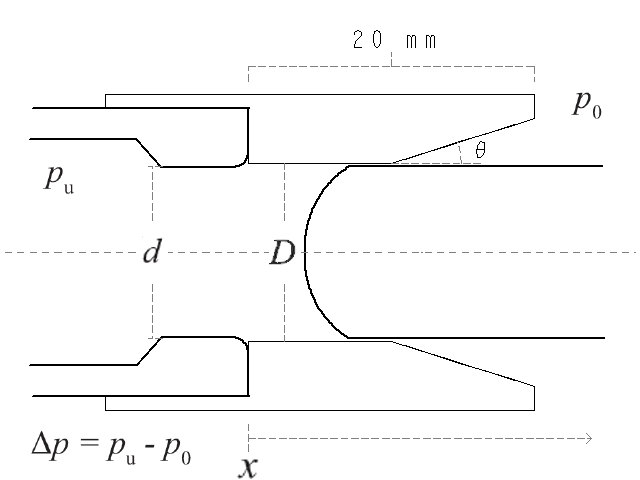
\includegraphics[scale=0.45]{Bilder/Method/ContactAndNozzleFunnelShape5.png}
\caption{The contact and nozzle for geometry \textit{a} and \textit{b}. The diameter of the contact is \textit{d}, and the inner diameter of the nozzle is \textit{D}.} \label{fig:contactAndNozzle}
\end{figure}

\begin{figure} [H] %denne må byttes ut.
\centering
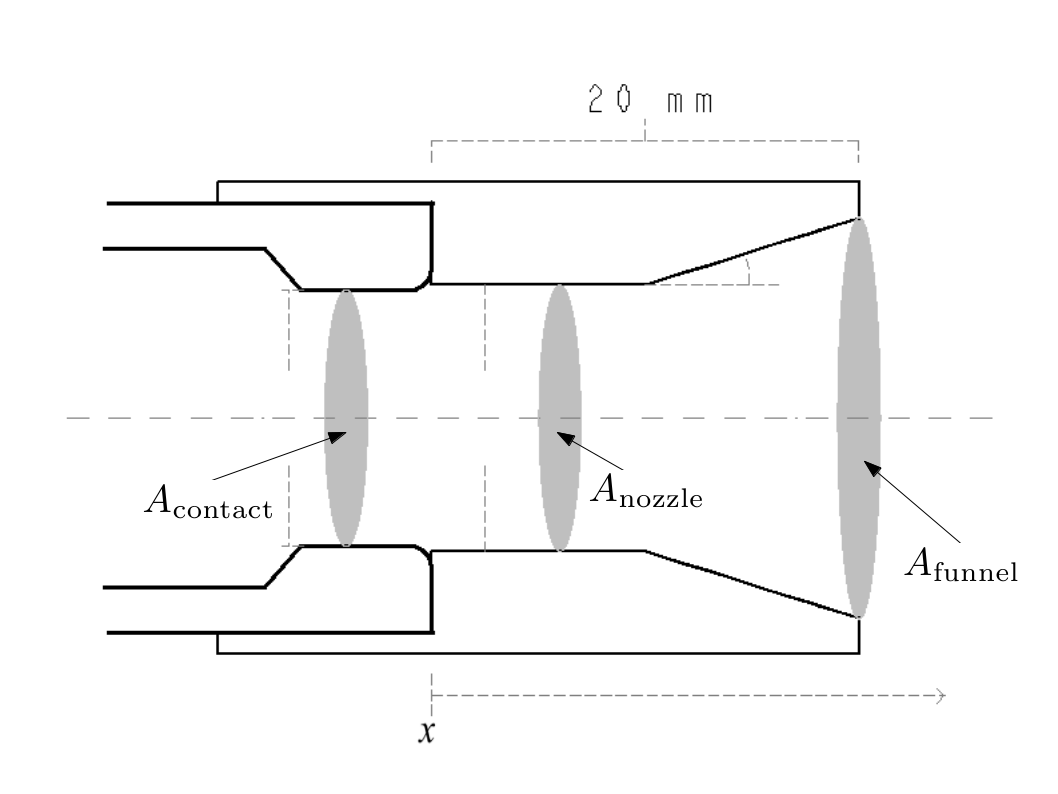
\includegraphics[scale=0.35]{Bilder/Method/AreaDef.png}
\caption{Overview of the definitions of the areas.} \label{fig:AreacontactAndNozzle}
\end{figure}

\newpage
For geometry \textbf{a} and \textbf{b} the following definitions apply:
\begin{itemize}
\item $A_\mathrm{{contact}}$ is the cross section of the contact pin, as well as the area of the tulip contact. The area is described by equation \eqref{eq:A_contact}.

\item $A_\mathrm{{nozzle}}$ is defined as the area of the cylindrical part of the nozzle, where x=[0,10] mm. The area is described by equation \eqref{eq:A_nozzle}.

\item $A_\mathrm{{funnel}}$ is defined as the area at the end of the nozzle, where x=20 mm, and the diameter of the funnel is at its largest. This area is described by equation \eqref{eq:A_funnel}.

\item The angle $\mathrm{\theta}$ is defined so that $A_\mathrm{{funnel}}=4 \cdot A_\mathrm{{nozzle}}$ for each geometry.

\item $A_\mathrm{{ring}}$ is in table \ref{tab:contGeoPara} defined as the area between the pin contact and the cylindrical part of the nozzle, where x=[0,10] mm, and is described by equation \eqref{eq:A_ring_1}. For x=[10,20] mm, $A_\mathrm{{ring}}$ is a function of the pin's position, x, inside the nozzle, described by equation \eqref{eq:A_ring_2}.
\end{itemize}

\begin{equation} \label{eq:A_contact}
A_\mathrm{{contact}}=A_\mathrm{{tulip}}=\pi \frac{d^2}{4}
\end{equation}
\begin{equation} \label{eq:A_nozzle}
A_\mathrm{{nozzle}}=\pi \frac{D^2}{4}
\end{equation}

\begin{equation} \label{eq:A_funnel}
A_\mathrm{{funnel}}=4 \cdot A_\mathrm{{nozzle}}=4\pi \frac{D^2}{4}
\end{equation}

\begin{equation} \label{eq:A_ring_1}
A_\mathrm{{ring}}=A_\mathrm{{nozzle}}-A_\mathrm{{contact}}=\pi\left( \frac{D^2}{4}-\frac{d^2}{4}\right)
\end{equation}
\begin{equation} \label{eq:A_ring_2}
A_\mathrm{{ring}}(x)=\pi\left( \left(\frac{2(x-10)\tan \theta + D}{2}\right)^2-\frac{d^2}{4}\right)
\end{equation}

\begin{table}[H]
\center
\caption{Contact geometry parameters for the funnel shaped nozzle design.}
 \begin{tabular}{|c|c|c|c|c|c|c|c|c|}
\hline 
Geometry & \textit{D} & \textit{d}  & $\frac{D}{d}$ & $\mathrm{\theta}$ & $A_\mathrm{{contact}}$ & $A_\mathrm{{ring}}$  & $A_\mathrm{{nozzle}}$ & $A_\mathrm{{funnel}}$ \\
  & [mm] &  [mm] &   &   &   [mm$^2$] &  [mm$^2$] &   [mm$^2$] &   [mm$^2$]\\
\hline 
\textbf{a} & 6.25 & 6.0 & 1.04 & 17.4 & 28.3 & 2.4 & 30.7 & 122.8\\ 
\hline 
\textbf{b} & 7.40 & 7.1 & 1.04 & 20.3 & 39.6 & 3.4 & 43.0 & 172.0\\ 
\hline 
\end{tabular} 
\label{tab:contGeoPara}
\end{table}

In figure \ref{fig:contactAndNozzleC} the contact geometry denoted \textbf{c} is presented. The length of the nozzle is 30 mm, and axial symmetry is present along the x-axis. The diameter of the contact is \textit{d} and the nozzle diameter is \textit{D}. The dimensions for the geometry is given in table \ref{tab:contGeoParaC}. $A_\mathrm{{contact}}$ and $A_\mathrm{{nozzle}}$ is defined in the same way as for geometry \textbf{a} and \textbf{b}, as presented in equation \eqref{eq:A_contact} and \eqref{eq:A_nozzle}. Since the nozzle is cylindrical for its entire length (x=[0,30] mm) $A_\mathrm{{funnel}}$ does not exist. Therefore, is $A_\mathrm{{ring}}$ defined as in equation \eqref{eq:A_ring_1} for x=[0,30] mm. 

As stated in section \ref{sec:puffer} a LBS design is often a scaled down version of a circuit breaker design. Therefore, a common contact diameter is $\approx$ 11 mm. However, test results presented in the paper "Air flow investigation for a medium voltage load break switch" have suggested that the optimal contact diameter depends on the current passing through the switch. In the paper mentioned above, tests for another geometry (denoted \textbf{d} in this report) which has the same $\frac{D}{d}$ as geometry \textbf{c}, has been conducted. These results is going to be compared with the interruption results for geometry \textbf{c}. Geometry \textbf{d} has a \textit{d}=6.0 mm, which seems to be the optimal value for a current of 630 A. Form these results Nina Sasaki Aanensen has calculated that the optimal contact diameter for a current of 880 A is 7.1 mm. Therefore, this value has been selected for \textit{d} to geometry \textbf{c}.

\begin{figure} [H]
\centering
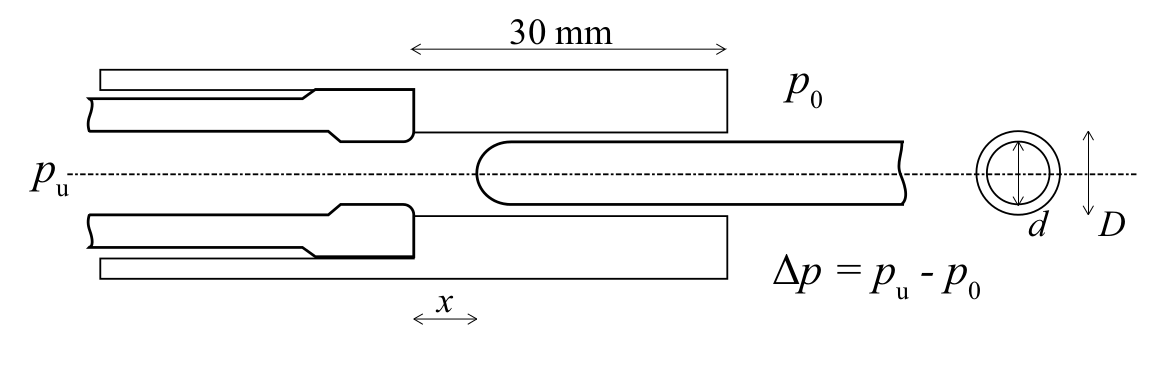
\includegraphics[scale=0.3]{Bilder/Method/contactSetUp.png}
\caption{The contact and nozzle for geometry \textbf{c}. The diameter of the contact is \textit{d}, and the inner diameter of the nozzle is \textit{D} \cite{bib:AFIMVLBA}.} \label{fig:contactAndNozzleC}
\end{figure}

\begin{table}[H]
\center
\caption{Contact geometry parameters for the cylindrical shaped nozzle design.}
 \begin{tabular}{|c|c|c|c|c|c|c|}
\hline 
Geometry & \textit{D} & \textit{d}  & $\frac{D}{d}$ &  $A_\mathrm{{contact}}$ & $A_\mathrm{{ring}}$  & $A_\mathrm{{nozzle}}$ \\
  & [mm] &  [mm] &   &  [mm$^2$] &  [mm$^2$] &   [mm$^2$] \\
\hline 
\textbf{c} & 9.6 & 7.1 & 1.35 & 39.6 & 32.8 & 72.4 \\ 
\hline
\end{tabular} 
\label{tab:contGeoParaC}
\end{table}

\subsection{Procedure}
Interruption tests with CZ occurring both inside and outside the nozzle are carried out. Six tests in total are conducted in this interruption experiment. One test consists of one contact geometry at a current magnitude of either 630 A or 880 A with a minimum of:
\begin{itemize}
\item For geometry \textbf{a} and \textbf{b}: \\
Five interruptions inside the funnel part of the nozzle and five interruptions outside the nozzle at each pressure level.

\item For geometry \textbf{c}: \\
Five interruptions outside the nozzle at each pressure level.

\end{itemize}
At least three different pressure levels are included in each test. Both the first and second CZ are included in this study in order to provide as much data as possible.

For geometry \textbf{a} and \textbf{b} "inside funnel" is defined as contact position x = [10, 20] mm and "outside nozzle" as x = [20, 60] mm at first CZ. Results from zero crossings that occurs in the cylindrical part of the nozzle, x $<$ 10 mm, between the tulip contact and the start of the funnel-shaped nozzle are discarded. For geometry \textbf{c} "outside nozzle" is defined as x = [30, 60] mm at first CZ. Interruptions that occurs "inside nozzle", x $<$ 30 mm, for geometry \textbf{c} are discarded. The first CZ occurs within x $<$ 60 mm, and the second CZ occurs for x $>$ 60 mm, as the contact speed during all tests is 5.5 mm/ms $\pm$ 0.5 mm/ms. When testing the interrupting capabilities inside the funnel, the first CZ is aimed to occur at x=15 mm. When testing outside the nozzle, the first CZ is aimed at x=30 mm for geometry \textbf{a} and \textbf{b} and x=45 mm for geometry \textbf{c}. Due to variation in the travelling speed of the contacts, some difference in the position of the pin at the moment of CZ will occur between each interruption attempt.
\newpage
When testing the interrupting capabilities, the test procedure for each of the six cases is as follows: 

\begin{itemize}
\item[1.] A pressure level that seems to be in the area of interest is found by performing some initial test interruptions at different pressure levels. This level is kept constant for at least five interruption tests.
\item[2.] If a pressure level results in less than 100\% successful interruptions, at least five new tests with a higher upstream pressure (next level) are conducted. This is repeated until at least one pressure level with five successful interruptions is found.
\item[3.] Then, the pressure is stepped down until 60\% or more of the interruption attempts fail, or the lowest possible pressure level is tested.
\end{itemize}

When testing for variations in the arcing voltage between a successful and unsuccessful interruption, a pressure level where the interruption success rate is 50 \% is used. Then, five successful interruptions and five unsuccessful interruptions are obtained while the arcing voltage is measured and stored for further use. All the interruptions should occur outside the nozzle. The switching process is filmed by a NIR high-speed camera so that the path of the arc can be monitored during the interruption.

The pin is cleaned, polished, and greased between each test to ensure a smooth surface. The contacts and nozzle are replaced regularly to avoid contact wear and nozzle deformation. This is to ensure that the geometry is constant through the whole experiment.
\cleardoublepage

\section{Results}
\subsection{Interruption tests} 


\newpage
\subsection{Arcing voltage}


\newpage
\subsection{Durability of the arcing contacts} \label{sec:durability}



\cleardoublepage

\section{Discussion}
\subsection{The probability of interruption} 


\subsection{Arcing voltage considerations}
 

\subsection{Durability of the arcing contacts} \label{fig:durability}


\newpage
\subsection{Suggestion for further work}
\subsubsection{A nozzle that minimises arc impact on air flow}


\subsubsection{Cone-shaped nozzle}


\cleardoublepage

\section{Conclusion}


\cleardoublepage
\begin{thebibliography}{10}
\bibitem{bib:SF6PI} L.G. Christophorou, J. K. Olthoff, and R.J. Van Brunt, "Sulfur hexafluoride and the electric power industry", \textit{IEEE Electrical Insulation Magazine, vol. 13, No. 5, pp. 20-24}, Oct. 1997.

\bibitem{bib:comSub} amesimpex.com, \url{http://www.amesimpex.com/images/unitised_sub_002.jpg}, 26.9.2013

\bibitem{bib:HVEbreak} M. Runde, "Current interruption in power grids", Trondheim: Norwegian University of Science and Technology, 2013

\bibitem{bib:GFALEAPI} E. Attar, P. Skryten, T. R. Bjortuft, P. Stoller, N. Ranjan, O. Granhaug, M. Schwinne and B. Wuethrich "Gas flow analysis in low energy arc puffer interrupters", \textit{22$^{nd}$ International Conference on Electricity Distribution CIRED, NO. 0410}, June 2013.

\bibitem{bib:CBAC} W. Rieder, "Circuit breakers, physical and engineering problems, III-Arc-medium considerations", \textit{IEEE spectrum, pp. 80-84}, Sept. 1970.

\bibitem{bib:IPSF6AQM} W. Hertz, H. Motschmann and H. Wittel, "Investigations of the properties of SF$_6$ as an arc quenching medium", \textit{Proceedings of The IEEE, vol. 59, NO. 4, pp. 485-492}, April 1971.

\bibitem{bib:TDCIGBB} W. Hermann, "Theoretical description of the current interruption in HV gas blast breakers", \textit{IEEE Transactions on Power Apparatus and System, vol. PAS-96, NO. 5, pp. 1546-1555}, Sept./ Oct. 1977.

\bibitem{bib:CIHVN} G. Frind and B. W. Swanson "Current Interruption in High-Voltage Networks", Baden: BBC Brown, Boveri \& Company Limited, 1977

\bibitem{bib:THFD} R. W. Johnson, "The handbook of fluid dynamics", Heidelberg: Springer-Verlag GmbH \& Co. KG, 1998.

\bibitem{bib:TET4160HVIM} E. Ildstad, "High voltage insulation materials", Trondheim: Norwegian University of Science and Technology, 2012, August 2012.

\bibitem{bib:KlimaKur2020} "KLIMAKUR2020", Oslo: Klima- og forurensningsdirektoratet, 2010

\bibitem{bib:consSF6} esrl.noaa.gov, \url{http://www.esrl.noaa.gov/gmd/webdata/iadv/ccgg/graphs/pdfs/ccgg.MLO.sf6.1.none.discrete.all.pdf}, 17.10.2013

\bibitem{bib:regSF6Miljo} regjeringen.no, \url{http://www.regjeringen.no/nb/dep/md/dok/regpubl/stmeld/2011-2012/meld-st-21-2011-2012/5/5.html?id=682932}, 21.10.2013

\bibitem{bib:StatSF6} K. L. Hansen, "Emissions from consumption of HFCs, PFCs and SF$_6$ in Norway", \textit{Statistics Norway/Department of Economic Statistics/Environmental Statistics}, 2007.

\bibitem{bib:AFIMVLBA} N. S. Aanensen, E. Jonsson, and M. Runde "Air flow investigation for a medium voltage load break switch", to be published.

\bibitem{bib:CIAMVLBS} E. Jonsson, N. S. Aanensen and M. Runde, "Current interruption in air for a medium voltage load break switch", \textit{IEEE Trans. Power Delivery}, in press.

\end{thebibliography}

\cleardoublepage
\appendix
\vspace*{\fill}
\begingroup
\begin{center}
\huge Appendix
\end{center}
\endgroup
\vspace*{\fill}
\cleardoublepage
\section{Appendix: Test Results} \label{app:rawData}
\setcounter{figure}{0}
\makeatletter 
\renewcommand{\thefigure}{A.\@arabic\c@figure}
\makeatother

\setcounter{table}{0}
\makeatletter 
\renewcommand{\thetable}{A.\@arabic\c@table}
\makeatother

\subsection{400 A geometry \textit{a} and \textit{b}} \label{app:testResults400A} 

\subsection{630 A geometry \textit{a} and \textit{b}} \label{app:testResults630A}

\newpage



\cleardoublepage
\section{Appendix: Previous relevant experiment} \label{app:PrevReleEx}
\makeatletter 
\renewcommand{\thefigure}{B.\@arabic\c@figure}
\makeatother

\makeatletter 
\renewcommand{\thetable}{B.\@arabic\c@table}
\makeatother

\section{Appendix: Matlab code for sortVoltage.m} %husk å oppdatere denne!!
\lstinputlisting[language=Matlab]{sortVoltage.m}

\end{document}
